%%!TEX encoding = UTF-8 Unicode

% According to UA rules, font size should range from 10 to 12pt.
\documentclass[11pt,a4paper,openright,final,twoside,onecolumn]{memoir}

\listfiles
\fixpdflayout

\usepackage[utf8]{inputenc}

% Computer Modern Typewritter (For bold ttfamily in listings)
\usepackage{lmodern}
% OR... Bera Mono
%\usepackage[scaled]{beramono} % TTT Font
%\usepackage{anyfontsize} % As the name says...

\usepackage[T1]{fontenc}

% For Overleaf support
\usepackage{ifthen}
\def\useoverleaf{0}  % change to non-zero (for instance, 1) to enable it

\makeatletter
\newcommand{\makecoverfile}[0]{%
  \immediate\write18{latexmk -pdf cover.tex}%
}
\makeatother

%For PDF merging
\usepackage{pdfpages}

%SET DPI to 300
\pdfpxdimen=\dimexpr 1in/300\relax

\usepackage{morewrites} % Allow the use of a larger number of packages

%For English and Portuguese languages
%Portuguese will be the default.
%Use \setdefaultlanguage to change it
\usepackage{csquotes}
\usepackage[english,portuguese]{babel}

% For custom date format
\usepackage{datetime}
\newdateformat{thesisdate}{\monthname[\THEMONTH] \THEYEAR} % Month Year

\usepackage{microtype} % Make pdf look better

\usepackage{booktabs} % for tables
\usepackage{lscape} % horizontal tables

% Uncomment to enable floats on facing pages
%\usepackage{dpfloat}

%Side by side figures
% Eg. Fig 1a, Fig 1b
\usepackage[hang,small,bf]{caption}
%\let\tion\undefined
%\let\subfloat\undefined
\usepackage{subcaption}

%\RequirePackage{textcase}

% Dropped Caps
%\usepackage{lettrine}


% Configure Hyperlink color
%\usepackage[breaklinks=true,colorlinks=false,linkcolor=blue]{hyperref}
% Or use the default
\usepackage{hyperref}

%Optional: Redefine section names
%\def\sectionautorefname{Section}
%\def\chapterautorefname{Chapter}
%\def\figureautorefname{Figure}
%\def\listingautorefname{Listing}
%\def\tableautorefname{Table}

%For PDF Comments
\usepackage{comment}
\usepackage{pdfcomment}
\usepackage{bookmark} % New Bookmarks

%For Multiple columns in Glossary
\usepackage{multicol}

%Math symbols
\usepackage{amsmath}
\usepackage{amssymb}

%Graphics
\usepackage{graphicx}

%Colors
\usepackage{xcolor}

%Euro symbol
\usepackage{eurosym}

% Code boxes
\ifthenelse{\equal{\useoverleaf}{0}}
{\usepackage[outputdir=build]{minted}}
{\usepackage{minted}}%

\renewcommand\listingscaption{Código}
\fvset{fontsize=\footnotesize} % Make Code blocks smaller than text

%Biber using IEEE style for proper UTF-8 support
\usepackage[backend=biber,style=ieee, sorting=none]{biblatex}
\bibliography{bib/references.bib}

%Use acronyms
\usepackage[printonlyused]{acronym} % For acronyms

% Enable chart support through pgf and tikz
\usepackage[version=0.96]{pgf}
\usepackage{tikz}
\usepackage{pgf-umlsd}
\usetikzlibrary{arrows,shadows,trees,shapes,snakes,automata,backgrounds,petri,mindmap} % for pgf-umlsd

%For Electric Circuits
\usepackage[detect-weight=true, binary-units=true]{siunitx}
\sisetup{load-configurations = binary}

\usepackage[american,cuteinductors,smartlabels]{circuitikz}

\usetikzlibrary{calc}
\ctikzset{bipoles/thickness=1}
\ctikzset{bipoles/length=0.8cm}
\ctikzset{bipoles/diode/height=.375}
\ctikzset{bipoles/diode/width=.3}
\ctikzset{tripoles/thyristor/height=.8}
\ctikzset{tripoles/thyristor/width=1}
\ctikzset{bipoles/vsourceam/height/.initial=.7}
\ctikzset{bipoles/vsourceam/width/.initial=.7}
\tikzstyle{every node}=[font=\small]
\tikzstyle{every path}=[line width=0.8pt,line cap=round,line join=round]

% For inline TT text (e.g. code snippets)
\usepackage{verbatim}

% For identing the first paragraph after section start
\usepackage{indentfirst}

 %Frames around figures and allow force placement
\usepackage{float}

%Configure Float style
%\floatstyle{boxed}
%\restylefloat{table}
%\restylefloat{figure}
%\restylefloat{lstlisting}

%For test purposes
\usepackage{lipsum}

%Keep floats inside section!
\usepackage[section]{placeins}
\let \oldsubsubsection \subsubsection
\renewcommand{\subsubsection}[2][]{
  \FloatBarrier
  \oldsubsubsection#1{#2}
}
\let \oldsubsection \subsection
\renewcommand{\subsection}[2][]{
  \FloatBarrier
  \oldsubsection#1{#2}
}
\let \oldsection \section
\renewcommand{\section}[2][]{
  \FloatBarrier
  \oldsection#1{#2}
}
\let \oldchapter \chapter
\renewcommand{\chapter}[2][]{
  \FloatBarrier
  \oldchapter#1{#2}
}


%%%% Use the built-in division styling
\headstyles{memman}

%%% ToC down to subsections
\settocdepth{subsection}

%%% Numbering down to subsections as well
\setsecnumdepth{subsection}

%%%% extra index for first lines
\makeindex[lines]

%Margins for University of Aveiro Thesis
\setlrmarginsandblock{3cm}{2.5cm}{*}
\setulmarginsandblock{3cm}{3cm}{*}
\checkandfixthelayout

%Or custom spacing
%\addtolength{\parskip}{0.5\baselineskip}
\linespread{1.5}

\begin{document}
\ifthenelse{\equal{\useoverleaf}{0}}{}{\makecoverfile{}}%
\includepdf[pages=-]{cover.pdf}

%
%Front matter

%Custom Chapter style named thesis
\makechapterstyle{thesis}{% Based on ell
  \chapterstyle{default}
  \renewcommand*{\chapnumfont}{\normalfont\sffamily}
  \renewcommand*{\chaptitlefont}{\normalfont\Huge\sffamily}
  \settowidth{\chapindent}{\chapnumfont 111}
  \renewcommand*{\chapterheadstart}{\begingroup
    \vspace*{\beforechapskip}%
    \begin{adjustwidth}{}{-\chapindent}%
    \hrulefill
    \smash{\rule{0.4pt}{15mm}}
    \end{adjustwidth}\endgroup}
  \renewcommand*{\printchaptername}{}
  \renewcommand*{\chapternamenum}{}
  \renewcommand*{\printchapternum}{%
    \begin{adjustwidth}{}{-\chapindent}
    \hfill
    \raisebox{10mm}[0pt][0pt]{\fontsize{30}{25}\selectfont\chapnumfont \thechapter}%
                              \hspace*{1em}
    \end{adjustwidth}\vspace*{-3.0\onelineskip}}
  \renewcommand*{\printchaptertitle}[1]{%
    \vskip\onelineskip
    \raggedleft {\chaptitlefont ##1}\par\nobreak\vskip 4\onelineskip}}

%Select chapter style from existing or select custom
%\chapterstyle{thesis} % Others: dowding, demo2, dash, chappell, brotherton, bianchi, ger, madsen, tatcher, veelo,indexes)
% thesis can also be used as defined previously
%

%If you feel adventurous you can also define all aspects of your theme
%Use either this input or the chapterstyle before
%% Rules
\newcommand{\thinRule}{\rule{\textwidth}{0.25pt}}

% Customize heading appearances
% Define styles
\newcommand{\partSize}{\Huge}
\newcommand{\partStyle}{\lsstyle\scshape}
\newcommand{\chapterSize}{\Huge}
\newcommand{\chapterStyle}{\lsstyle\scshape}
\newcommand{\chapterAfter}{}
\newcommand{\sectionSize}{\Large}
\newcommand{\sectionStyle}{\scshape\MakeTextLowercase}
\newcommand{\subsectionSize}{\large}
\newcommand{\subsectionStyle}{\scshape\MakeTextLowercase}
\newcommand{\subsubsectionSize}{\large}
\newcommand{\subsubsectionStyle}{\scshape\MakeTextLowercase}
\newlength{\partNumSizePt}
\setlength{\partNumSizePt}{60pt}
\newlength{\chapterNumSizePt}
\setlength{\chapterNumSizePt}{60pt}
\newcommand{\partNumSize}{%
  \fontsize{\partNumSizePt}{1.2\partNumSizePt}\selectfont%
}
\newcommand{\partNumStyle}{\partChapterNumColor}
\newcommand{\chapterNumSize}{%
  \fontsize{\chapterNumSizePt}{1.2\chapterNumSizePt}\selectfont%
}
\newcommand{\chapterNumStyle}{\partChapterNumColor}

% Customize parts
\renewcommand{\partnamefont}{\partSize\partStyle}
\renewcommand{\partnumfont}{\partNumSize\partNumStyle}
\renewcommand{\printpartname}{}
\renewcommand{\printparttitle}[1]{%
  \normalfont\normalcolor\partnamefont #1
}

% Customize chapters
\makeatletter
\setlength{\beforechapskip}{30pt}
\renewcommand*{\chapterheadstart}{\vspace*{\beforechapskip}}
\setlength{\afterchapskip}{3ex}
\setlength{\midchapskip}{3ex}
\renewcommand*{\chapnamefont}{%
  \Large\flushright\chapterStyle\partChapterNumColor%
}
\renewcommand*{\chapnumfont}{\chapterNumSize\chapterNumStyle}
\renewcommand*{\chaptitlefont}{%
  \normalfont\flushleft\normalcolor\chapterSize\chapterStyle%
}
\renewcommand*{\printchaptername}{%
  \chapnamefont\MakeTextLowercase{\@chapapp}%
}
\renewcommand*{\chapternamenum}{\quad}
\renewcommand*{\printchapternum}{%
%  \chapnumfont\textls[-75]{\classicstylenums{\thechapter}}%
 \chapnumfont\textls[-75]{\thechapter}%

}
\renewcommand*{\printchaptertitle}[1]{%
  \chaptitlefont #1
  \chapterAfter
}
\makeatother
% Customize sections and subsections
\setsecnumformat{\csname my#1\endcsname\quad}
\setsecheadstyle{\sectionSize\sectionStyle}
\newcommand{\mysection}{{\thesection}}
\setlength{\beforesecskip}{3em}


\setsubsecheadstyle{\subsectionSize\subsectionStyle}
\newcommand{\mysubsection}{{\normalfont\subsectionSize\thesubsection}}
\setlength{\beforesubsecskip}{3em}

\setsubsubsecheadstyle{\subsubsectionSize\subsubsectionStyle}
\newcommand{\mysubsubsection}{{\normalfont\subsubsectionSize\thesubsubsection}}
\setlength{\beforesubsubsecskip}{2em}

% Customize "Table of ..." appearance
% Customize headings
\newcommand{\renewPrintXTitle}[1]{%
  \renewcommand{#1}[1]{%
    \printchaptertitle{##1}%
  }%
}
\renewPrintXTitle{\printtoctitle}
\renewPrintXTitle{\printlottitle}
\renewPrintXTitle{\printloftitle}

% Customize ToC headings
\renewcommand{\cftpartfont}{\partChapterNumColor\partStyle}
\renewcommand{\cftchapterfont}{\chapterStyle}
\renewcommand{\cftsectionfont}{}
\renewcommand{\cftsubsectionfont}{}
\renewcommand{\cftfigurefont}{}
\renewcommand{\cfttablefont}{}
\newcommand{\cftlstlistingfont}{}

% Increase number width
\newlength{\cftNumWidthIncrease}
\setlength{\cftNumWidthIncrease}{0.25em}
\addtolength{\cftpartnumwidth}{\cftNumWidthIncrease}
\addtolength{\cftchapternumwidth}{\cftNumWidthIncrease}
\addtolength{\cftsectionindent}{\cftNumWidthIncrease}
\addtolength{\cftsubsectionindent}{\cftNumWidthIncrease}
% No leader dots
%\renewcommand*{\cftpartdotsep}{\cftnodots}
%\renewcommand*{\cftchapterdotsep}{\cftnodots}
%\renewcommand*{\cftsectiondotsep}{\cftnodots}
%\renewcommand*{\cftsubsectiondotsep}{\cftnodots}
%\renewcommand*{\cftfiguredotsep}{\cftnodots}
%\renewcommand*{\cfttabledotsep}{\cftnodots}
%\newcommand*{\cftlstlistingdotsep}{\cftnodots}
% Set page numbers immediately after entry text
\newcommand{\tocEntryPageSep}{\hspace{1em}}
\renewcommand{\cftpartleader}{\cftdotfill{\cftdotsep}}
%\renewcommand{\cftpartafterpnum}{\cftparfillskip}
%\renewcommand{\cftchapterleader}{\tocEntryPageSep}
\renewcommand{\cftchapterleader}{\cftdotfill{\cftdotsep}}
%\renewcommand{\cftchapterafterpnum}{\cftparfillskip}
\renewcommand{\cftsectionleader}{\cftdotfill{\cftdotsep}}
%\renewcommand{\cftsectionafterpnum}{\cftparfillskip}
\renewcommand{\cftsubsectionleader}{\cftdotfill{\cftdotsep}}
%\renewcommand{\cftsubsectionafterpnum}{\cftparfillskip}
\renewcommand{\cftfigureleader}{\cftdotfill{\cftdotsep}}
%\renewcommand{\cftfigureafterpnum}{\cftparfillskip}
\renewcommand{\cfttableleader}{\cftdotfill{\cftdotsep}}
%\renewcommand{\cfttableafterpnum}{\cftparfillskip}
\newcommand{\cftlstlistingleader}{\cftdotfill{\cftdotsep}}
%\newcommand{\cftlstlistingafterpnum}{\cftparfillskip}
% Customize page numbers
\newcommand{\tocPageStyle}{\tocPageColor}
\renewcommand{\cftpartpagefont}{\tocPageStyle}
\renewcommand{\cftchapterpagefont}{\tocPageStyle}
\renewcommand{\cftsectionpagefont}{\tocPageStyle}
\renewcommand{\cftsubsectionpagefont}{\tocPageStyle}
\renewcommand{\cftfigurepagefont}{\tocPageStyle}
\renewcommand{\cfttablepagefont}{\tocPageStyle}
\newcommand{\cftlstlistingpagefont}{\tocPageStyle}

% Abstract
% Remove indents around abstract text
\setlength{\absleftindent}{0pt}
\setlength{\absrightindent}{0pt}
% Change font size to conform with the rest of the document text
\renewcommand{\abstracttextfont}{\normalsize}

% Customize headers and footers including page numbers
\newcommand{\hfTextSize}{\footnotesize}
\newcommand{\headTextStyle}{\lsstyle\scshape\MakeTextLowercase}
\nouppercaseheads
\makeevenhead{headings}%
             {\hfTextSize\thepage}%
             {}%
             {\hfTextSize\headTextStyle\leftmark}
\makeevenhead{plain}%
             {\hfTextSize\thepage}%
             {}%
             {\hfTextSize\headTextStyle\leftmark}
\makeoddhead{headings}%
            {\hfTextSize\headTextStyle\rightmark}%
            {}%
            {\hfTextSize\thepage}
\makeoddhead{plain}%
            {\hfTextSize\headTextStyle\rightmark}%
            {}%
            {\hfTextSize\thepage}


% Customize captions
\newcommand{\captionSize}{\small}
\newcommand{\captionStyle}{\scshape}
\newcommand{\captionWidthRatio}{0.9}

\captionnamefont{\captionSize\captionStyle}
\captiontitlefont{\captionSize}
\captiondelim{ -- }
\captiontitlefinal{}
\changecaptionwidth
%\captionwidth{\captionWidthRatio\textwidth}

% Define colors
%\newcommand{\titleColor}{\color[rgb]{0.616, 0.0627, 0.176}}
\newcommand{\titleColor}{\color[rgb]{0,0,0}}

\newcommand{\partChapterNumColor}{\titleColor}
\newcommand{\dropCapColor}{\titleColor}
%\newcommand{\tocPageColor}{\color[rgb]{0.0980, 0.329, 0.651}}

\newcommand{\tocPageColor}{\color[rgb]{0, 0,0}}
\definecolor{shade0}{rgb}{1.0 , 1.0 , 1.0 }
\definecolor{shade1}{rgb}{0.9 , 0.9 , 0.9 }
\definecolor{shade2}{rgb}{0.8 , 0.8 , 0.8 }
\definecolor{shade3}{rgb}{0.65, 0.65, 0.65}
\definecolor{shade4}{rgb}{0.45, 0.45, 0.45}
\definecolor{shade5}{rgb}{0.0 , 0.0 , 0.0 }



\chapterstyle{veelo}
%Exclude sub figures from List of Figures
%\captionsetup[subfloat]{list=no}


% Texts
\newenvironment{introduction}
{%
  \begin{minipage}{\textwidth}%
   \itshape%
}
{%
  \end{minipage}%
  \par\addvspace{2\baselineskip plus 0.2\baselineskip minus 0.2\baselineskip}%
}


%Select Page style
\pagestyle{plain}

\frontmatter

\tightlists
\midsloppy
\raggedbottom

\setcounter{tocdepth}{2} %subsections are added to the TOC
\setcounter{secnumdepth}{4} %subsubsections are numbered


\cleardoublepage

%Table of contents
{\small\tableofcontents}
\cleardoublepage

%List of figures
{\small\listoffigures}


%List of tables
\cleardoublepage
{\small\listoftables}

%Print Glossary
{\small\chapter{Glossário}

\footnotesize
\SingleSpacing

\begin{multicols}{2}
\begin{acronym}[AAAAAA]

	\acro{rfid}[RFID]{Radio Frequency Identification}
	\acro{rf}[RF]{radio frequency}
	\acro{lf}[LF]{Low Frequency}
	\acro{hf}[HF]{High Frequency}
	\acro{uhf}[UHF]{Ultra High Frequency}
	\acro{uwb}[UWB]{Ultra-wide band}
	\acro{uhfrfid}[UHF RFID]{Ultra High Frequency Radio Frequency Identification}
	\acro{cps}[CPS]{Cyber-physical Systems}
	\acro{iot}[IoT]{Internet of Things}
	\acro{it}[IT]{Information Technology}
	\acro{ucc}[UCC]{Uniform Code Council}
	\acro{ean}[EAN]{European Article Number}
	\acro{unspsc}[UNSPSC]{United Nations Standard Products and Services Code}
	\acro{undp}[UNDP]{United Nations Development Programe}
	\acro{gdsn}[GDSN]{Global Data Synchronisation Network}
	\acro{epc}[EPC]{Electronic Product Code}
	\acro{xml}[XML]{Extensible Markup Language}
	\acro{edi}[EDI]{Electronic Data Interchange}
	\acro{dod}[DoD]{United States Department of Defense}
	\acro{llrp}[LLRP]{Low Level Reader Protocol}
	\acro{fc}[F\&C]{Filter and Collection}
	\acro{c1g2}[C1G2]{Generation 1 Class 2}
	\acro{mit}[MIT]{Massachusetts Institute of Technology}
	\acro{iff}[IFF]{Identify Friend or Foe}
	\acro{us}[U.S.]{United States of America}
	\acro{rnd}[R\&D]{research and development}
	\acro{ocr}[OCR]{optical character recognition}
	\acro{em}[EM]{electromagnetic}
	\acro{emf}[EMF]{electromagnetic field}
	\acro{emw}[EMW]{electromagnetic wave}
	\acro{scm}[SCM]{Supply Chain Management}
	\acro{nfc}[NFC]{Near-field communication}
	\acro{eirp}[EIRP]{Effective Isotropic Radiated Power}
	\acro{ic}[IC]{integrated circuit}
	\acro{cw}[CW]{continuous wave}
	\acro{fpga}[FPGA]{field-programmable gate array}
	\acro{tds}[TDS]{Tag Data Standard}
	\acro{uuid}[UUID]{universally unique identifier}
	\acro{c1g2}[C1G2]{Class 1 Generation 2}
	\acro{worm}[WORM]{write once read many}
	\acro{id}[ID]{identifier}
	\acro{pc}[PC]{Protocol Control bits}
	\acro{gen2}[Gen2]{Generation 2}
	\acro{tid}[TID]{Tag Identification}
	\acro{crc}[CRC]{Cyclic Redundancy Check}
	\acro{xpc}[XPC]{Extended Protocol Control}
	\acro{umi}[UMI]{User Memory Indicator}
	\acro{tid}[TID]{Tag identifier}
	\acro{xtid}[XTID]{Extended Tag identifier}
	\acro{mdid}[MDID]{Mask Designer Identifier}
	\acro{tmn}[TMN]{Tag Model Number}
	\acro{dsfid}[DSFID]{Data Storage Format Identifier}
	\acro{urn}[URN]{Universal Resource Name}
	\acro{uri}[URI]{Uniform Resource Identifier}
	\acro{ons}[ONS]{Object Name Service}
	\acro{gtin}[GTIN]{Global Trade Item Number}
	\acro{sgtin}[SGTIN]{Serialised Global Trade Item Number}
	\acro{sku}[SKU]{Stock Keeping Unit}
	\acro{nid}[NID]{Namespace Identifier}
	\acro{nss}[NSS]{Namespace-specific String}
\end{acronym}
\end{multicols}

}

%
%Main document starts here
%
\mainmatter



% Start of Thesis text ----------------------------------------------------------
%Line spacing: 1.5 pt
\OnehalfSpacing

% To talk:
% - Nespresso, their logistics and how can RFID help
% - grab nespresso example e estrapolar para outros markets
% - CTT, logistica, integração com amazon, how can RFID help
% - *escolas/hospitais: controlo de material disponível
% - Necessity of RFID globaly: optimizar transporte (contentores de transporte maritimo), data analisys for predictions, um tecnologia que unifica APIs de todas as empresas 
% - Benefícios de smart shelves e de que forma se encaixa no environment  

\chapter{Introduction}

\section{Background and Motivation}

The new industrial revolution is centered around data. Yet, the true extension of this reformation might not be fully understood.

From manufacturing to retail, information and communication technologies disrupted the understanding of what could be improved through the supply chain~\footnote{the sequence of processes involved in the production and distribution of a commodity~\cite{OxfordLanguagesGoogle}}. 
To grasp the advantages of \ac{rfid}, we have to understand its place with other technologies and how it can empower the relationship between manufacturing, transportation, logistics and retail.

The introduction of information and communication technologies in the manufacturing process, has been the foundation of Industry 4.0, which some people refer as the fourth industrial revolution~\cite{marrWhatIndustryHere}. It expanded the cyber-physical systems \footnote{a system in which a mechanism is controlled or monitored by computer-based algorithms} of the third industrial revolution and introduced \ac{iot}, cloud and cognitive computing.
The rise of wireless communications and the massification of data sensing in the manufacturing processes, allowed these technologies to enhance and optimize production processes, logistics operations and marketing strategies.

Adding \ac{iot} provided the network infrastructure for data transfer. Cloud computing enabled on-demand availability of \ac{it} resources, fast deployment times and more efficient management strategies. Cognitive computing contributed with computer vision, signal processing and tools to analyze and process large amounts of data for operational optimizations and pattern recognition.
These technologies support the modern digital end-to-end system of a business and its manufacturing processes.

\ac{uhfrfid} improves the developments made in \emph{Industry 4.0} by adding digital visibility of physical assets. But visibility inside a company is opaque to trading partners and vice versa. Visibility both inside and outside of the company is desirable. With \ac{epc} that is possible. Inside the company, physical objects can be digitalized, identified and wirelessly tracked. Outside, frontiers between company methods of operations and tools, can be abstracted in a common set of interfaces and standards that allows visibility of products outside company bounds and share of information between trading partners.
This achieves an end-to-end integration of the complete commercialization process, where data from billions of physical items can be shared through the internet, enabling businesses and consumers to identify, locate and engage each item.

% Santos: parece meio solto (se calhar meter um gráfico ou algo do género)
The future of \ac{rfid} seems promising. In 2016, 96\% of apparel retailers had plans to deploy tags on their products~\cite{hardgrave2016StateRFID}. The \ac{dod} requires that all contractors must use \ac{uhfrfid} identification since 2005~\cite{DODReleasesFinal}.In 2014, Impinj, Intel, Google and Smartrac teamed up to form RAIN RFID, an organization whose mission is to promote the adoption of \acs{epc} \ac{uhfrfid}. \ac{uhfrfid} can greatly improve transport systems with cost reductions, smaller inventory, faster transportation and routing troubleshooting, lower insurance rates and greater efficiency~\cite{oanaRFIDTechnologyContainers2013}.

% Santos: Isto não soa bem a acabar a secção
Development and standardization of \ac{uhfrfid} enables a symbiotic relation across the chain, connecting production, logistics, retail and client.

\section{Scope}

This dissertation intents to explore the implementation of smart shelve and software for retail inventory management systems following the global supply chain standards. 


% Smart Shevels: where they stand in the RFID chain, what they bring to the market

% Nespresso: present conditions, how smart shelves can help (logistics, supply chain)

% The proposed solution is a system around \textbf{smart shelving}. 

% The structure storing the products contains RFID antennas and readers that detect and read the tags attach to them. Those readers will let the platform know in real time the state of the product in stock.

% This system should handle the registration and verification of arriving stock and manage in real time warehouse products. 

%The product should integrate with the logistics management software used by the company, allowing the a real-time management off all the products, machine learning predictions and control of the product flow.

%The solution must be reliable and cheap to maintain. The initial investment should also be the smallest possible. 

%Nespresso is owned by Nestlé Nespresso S. A., one operational unit of the Nestlé Group, with headquarters in Lausanne, Switzerland~\cite{nespressowebsite}. (...)

%With the growing of the brand, the complexity in the logistics networks starts to compromise the management of the products down in the chain. 

%The categorization and verification of new inventory, inspection of the arrived goods from the transportation company, returns, control and management of stocks, are all attended by manual labour. 
%The manual labour is prone to errors, takes a lot of working time and interfacing with the management software isn't usually efficient.

%\section{Objectives}

%\begin{itemize}
  %\item \textbf{Prevent stock-outs:} get timely replenishment and optimizes in-store sales and management. Logistics companies deliver goods on time and according to delivery requirements;
  %\item \textbf{Reduce time and errors from manual labour:} counts, identification, misplacement and lost or stolen items;
  %\item \textbf{Help customers:} find and engage with the products they want;
  %item \textbf{Control:} who removes or checks out valuable items;
  %\item \textbf{Automatic information and management of stock:} the logistics lines automatically transmits and receives stock information;
  %\item \textbf{Smart physical storage:} automatic identification of goods in the warehouse/shelves, automatic matching of distribution requirements, improves the efficiency of goods storage;
  %\item \textbf{Acquisition technology:} After the goods enter the collection area, the collection equipment automatically identifies multiple items by collecting RFID tags, thereby efficiently completing the goods in and out of the warehouse, ensuring whether the physical and distribution requirements are consistent, and improving the efficiency of goods distribution;
  %\item \textbf{Real-time:} master the distribution of all goods in real time, accurately grasp the inventory situation, optimize the reasonable inventory, and grasp the status and changes of the warehouse environment in real time;
%\end{itemize}

\section{Outline}

\cleardoublepage
\chapter{Basic principles of RFID}

\section{Contextualization} \label{sec:contextualization}

The concept of identification using \ac{rf} dates back to the late 1930s.
By this time, the primitive biplanes made of wood and fabric used in Word War I, had evolved to all-metal monoplanes. They were capable of carrying heavy quantities of explosives and travel at hundreds of kilometers per hour, making the conventional method of visual identification of incoming aircrafts obsolete.
To counteract this issue, nations invested in research and development that culminated in the development of the microwave radar.
By the time of the World War II, both fronts were using radar technologies to detect approaching planes. 
Still, it remained the problem of identifying allied aircrafts from enemie ones~\footnote{The attack at Pearl Harbor in $1941$ was possible due to a mistaken assignment of incoming Japanese aircraft to an unrelated \ac{us} bomber flight.}.
The German aircraft force, \emph{Luftwaffe}, observed that as pilots rolled their planes, it would change the radio signal reflected back. With this ingeniously simple maneuver, they were capable of discriminate allied aircrafts, being roughly the first \ac{rfid} passive application.~\cite{dobkinRFRFIDSecond2012}

It was soon later that Watson-Watt, under a British project, developed the first active \ac{rfid} application to be used in \ac{iff} systems. An active \ac{rf} transmitter was attached to British planes, which on receiving radar signals from base stations, broadcasted a signal identifying the aircraft has allied.~\cite{HistoryRFIDTechnology}

% This established the core concept of today's systems that make this dissertation possible - the over the air identification of transponders~\footnote{a device that, upon receiving a signal, emits a different signal in response}.

The technology kept advancing through the 1950s and 1960s, mainly in the academic field, but with private companies starting to commercialize anti-theft systems based on 1-bit transponders~\footnote{a simple inductive RC resonant circuit that detects transponders in field by changes in the reader coil voltage~\cite{andreventuradacruzmarnotozuqueteIdentificacaoPorRFID2018}}.

In the 1970s the first \ac{rfid} patents were registered. Kudos to the active tag with rewritable memory and a passive transponder for door lockers. It was during this time that the \ac{us} National Laboratory of Los Alamos was commissioned, by the Energy Department, to develop a tracking system for nuclear materials. The system revolved around transponders in trucks that would transmit information to readers at the gates of secure facilities. The Agricultural Department also requested Los Alamos for an animal tracking system, which was designed in the \ac{uhf} band with passive transponders, marking the beginning of the \ac{uhfrfid} technology. These systems were also transposed by the same engineers to automated toll payment systems in the private industry~\cite{landtHistoryRFID2005, HistoryRFIDTechnology,casierAnalogCircuitDesign2011}.

In the 1980s there was a upsurge in investment, with private industries wagering in \ac{rfid}, fueled by the development of the personal computer and promises of the technology.
By the 1990s, deployments of \ac{rfid} systems had grown significantly. The necessity of compatibility and interaction between proprietary systems rose, being established the first industry standards. 

The 2000s followed the same maturation process with slow adoption in the late part of the decade. 
Despite the interest presented by retail giants like Wal-Mart, and investment by the \ac{dod}, compromises created by the \ac{rfid} industry didn't justified the commitment to the technology. The high cost for investment, technical performance difficulties, conflicting standards, security issues and privacy concerns made the investment stale~\cite{RFIDAdoptionStalls}. 
Companies had to strangle \ac{rnd} resources due to inexistent tools and complex implementations. Resources required to develop marketing and sales tools, which truly utilize the \ac{rfid} infrastructure to increase revenue, had to be allocated to deploying \ac{rfid} systems.
Devise economic strategies for suppliers to transit to \ac{rfid} also seemed to be a problem, since many ordinary companies don't have \ac{rnd} resources at all to begin with~\cite{gaudinSuppliersGainFailed2008}.
Another big issue was the standardization of coding schemes in \ac{rf} tags. The fight for dominance in the \ac{uhfrfid} market led to multiple coding standards and protocols that made inter-operation among vendor and suppliers infeasible, if not impossible.

In the last decade, despite the advancements in the industry and adoption by big apparel retailers like Zara, Decathlon and Marks \& Spencer~\cite{RFIDRetailApparel}, there are issues that inhibit wide-scale adoption of \ac{uhfrfid}. These problems will be further discussed in chapter two of this dissertation.

\section{\ac{rfid} System}

% Reader notes:
% Eu:   talk about the range denomination for systems? close range, long range, ...
%       maybe talk about read range dependance of things (see slides on UHF) - pass the practical considerations section to here as a subsection

\ac{rfid} is an identification technology that uses radio waves or electro-magnetic fields to automatically identify physical objects and collect data about them.
Generally, \ac{rfid} solutions start with a radio device called tag. The tag is attached to the object that needs to be identified. When such a object is presented in front of an antenna connected to a suitable \ac{rfid} reader, the tag transmits data to the reader via the reader antenna. The reader then forward the information through a communication channel to a software application running on a computer.

\begin{figure}[!ht]
    \centering
    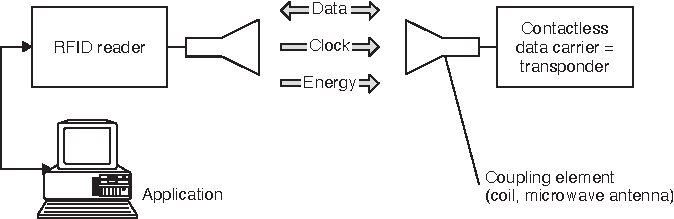
\includegraphics[width=0.8\textwidth]{./figs/02-state-of-the-art/rfid_system.pdf}
    \caption{\ac{rfid} system~\cite{finkenzellerRFIDHandbookFundamentals2003}} 
    \label{fig:rfidsystem}
\end{figure}

\subsection{Components}

An \ac{rfid} system is a collection of components that implement an \ac{rfid} solution.
Different references present different descriptions of \ac{rfid} systems. Many specify where and which components should be implemented.
The fact is, depending on the use case and requirements, these components can be implemented in different physical places or not implemented at all. With the current paradigm of \ac{iot}, machine learning and cloud computing, the discrimination of these components is even more difficult to establish. It is naive and intricate to predict what \ac{rfid} system architecture will be like in the next few years.

The component description of \ac{rfid} systems can be simplified to three physical blocks: \emph{Transponder} which is attached to the physical object to be identification, and is responsible for storing and transmitting appropriate data about the object; \emph{Reader} which interacts with transponders to read and write data; and \emph{Software system} that encompass all kinds of hardware and software components that are separated from the reader and support back-end infrastructures and business logic of a system.

From these, all components described in the literature can be specified and clearly added to one of the blocks.
The prevalent components used in \ac{rfid} systems:

\begin{description}
    \item[Tag] \ac{rf} device that can store and transmit data in a contactless manner using radio waves.
    \item[Reader] also called \emph{interrogator}, is a device that can read from and write data to compatible \ac{rfid} tags.
    \item[Reader Antenna] is a device that is attached to a reader and is responsible for the \ac{rf} interface with the tag.
    \item[Controller] is an interface that allows an external entity to communicate with and control a reader's functions and devices connected to it.
    \item[Sensor, actuator and annunciator] are optional components used for external input and output of the system.
    \item[Host and software system] is an term for all hardware and software components that are separated from the reader device (e.g.\ middleware, back-end infrastructure, point-of-sale terminals, etc.)
    \item[Communication infrastructure] is the wired and wireless network and serial connection infrastructure needed to connect the previously listed components
\end{description}

%\subsection{Advantages and Limitations}
%\subsection{Performance factors}
% read range dependance of transmitted power, ... ..

A run through the specificities of most of the components will be done in the following sections.

\section{\acl{em} Concepts} \label{sec:em}

% Readers Notes:
% - Edgar: no inicio parece que as regions são completamente separadas e só nas boundaries é que se percebe que é uma cena progressiva. Ver se re-radiating é uma cena "valida" ou arranjar uma melhor forma de dizer 
% - Eu: rever com o livro RFID Handbook pag. 102, melhorar a escrita, referenciar no texto as imagens e tabelas

Before presenting the intrinsics around \ac{rfid} system components, a basic expertise in \ac{em} concepts is paramount.
Designing well performant systems requires a good understanding of electromagnetism fundaments and its peculiarities.

In like manner to other wireless technologies, \ac{rfid} uses \acp{emf} or \acp{emw} as interface to transmit information back and forward between reader and transponder.
Engineers have to grasp how \acp{emf} and \acp{emw} behave within distance to the reader antenna, how materials in tagged objects can interfere with \ac{rf} signals, how unaccounted poor \ac{rf} environments can compromise deployment of \ac{rfid} systems, to say a few.

An \ac{emf} is the phenomenon produced by moving electric charges. It can be described through Maxwell's equations and mathematical abstracted as a combination of an electric field and a magnetic field that interact with each other and their surroundings.

The behavior of the fields changes as the distance from the source increases and are usually defined as two main regions: \emph{near-field} and \emph{far-field}. These regions separate \ac{rfid} technologies in a very concrete way, but should not misled to think that the boundaries are precisely defined. The regions change their behavior in a progressive manner. The rough discrimination between regions in \ac{rfid} exist to separate mutual coupling and radiation based technologies. 

\subsection{\emph{Near-field}}

\emph{Near-field} manifests from the electric and magnetic fields near the charges and current that directly produced them. It is the region where phenomena like \ac{em} induction and electrostatic occur.
This field can be further split in two regions: reactive \emph{near-field} and radiative \emph{near-field}.

%Due to the variation of the electric rotational field, a magnetic field with closed field lines occurs in space, called rotational field.
%It surrounds the electric field and itself varies over time thus generating another electric field.
%Due to the mutual dependance of the time varying fields there is a chain effect of electric and magnetic fields in space~\cite{finkenzellerRFIDHandbookFundamentals2003}. 

Is in the reactive region that \emph{near-field} \ac{rfid} technologies are defined for. It is the closest to the transmitting antenna and is characterized by non-radiative behaviors. In this region, if the energy is not absorbed by a receiver, self-capacitance and self-inductive effects cause the antenna to store energy very near its surface. When electrons from a nearby conductor are placed in this region, field reactive \emph{near-field} energy is transferred to them, resulting in an energy drain on the transmitter by a change in the impedance viewed by the reader~\cite{finkenzellerRFIDHandbookFundamentals2003, balanisAntennaTheoryAnalysis2005}.

In the radiative \emph{near-field}, i.e.\ Fresnel region, the back-coupling of the fields becomes out of phase with the antenna signal, and thus cannot efficiently return inductive or capacitive energy from antenna currents or charges.
In this region conductive objects, such as metal structures, can behave as antennas by inductively receiving and then \emph{re-radiating} some of the energy~\cite{ElectromagneticRadiationField}.

In the context of \ac{rfid} technologies, only the reactive zone is considered when referring to the \emph{near-field} region. The radiative zone is \textit{ineffective} and rather unpredictable and usually not accounted referring to \ac{rfid}.

The power of the field differers between field components with the distance ($d$) from the antenna. The magnetic field strength is proportional to $1/d^3$ and the electric to $1/d^2$. The \emph{near-field} components are quite powerful but usually only suited for close range \ac{rfid} technologies due to the rapid fall-off with the distance~\cite{balanisAntennaTheoryAnalysis2005}.

\subsection{\emph{Far-field}}

The \emph{far-field} region is the region where the \ac{em} field behaves as a \textit{normal} radiating field, composed of \ac{em} waves that propagate outwards - i.e.\ electromagnetic radiation.

\ac{em} waves are created as result of uniform vibrations between an electric field and a magnetic field. In other words, \ac{em} waves are composed of oscillating magnetic and electric fields. A change in one of the field components reflects an equal change of the other and one can not exist independently.
These waves are detached from any feedback from the moving charges that produced it. Means that, after the waves leave the transmitter, they are completely independent of both transmitter and receiver, as opposed to the phenomena in the \emph{near-field} region.

In this region the radiation amplitude decreases $1/d$ as the distance ($d$) from the reader antenna increases, being the suitable option for \ac{rfid} technologies requiring high reading distances (e.g.\ \ac{uhfrfid}).

\subsection{Boundaries}

The boundaries between these regions are characterized by locations where the activity of the associated field components are strongest. It does not mean that the other components aren't present, because they are. The transition between regions is progressive.

The \emph{near} and \emph{far fields} are roughly delimited by approximately one full wavelength of the \ac{rf} wave emitted from a reader antenna.
This can be more precisely defined taking in account the transmitting antenna characteristics.

For antennas whose size is comparable to wavelength or bigger (used in \ac{uhfrfid}), the \emph{far-field} boundary is delimited by the Fraunhofer distance, radial from the antenna. The Fraunhofer distance is described by $2D^2 / \lambda$, where $D$ is the largest dimension of the radiator and $\lambda$ the wavelength~\cite{balanisAntennaTheoryAnalysis2005}.
A representation of the borders between regions can be seen in figure~\ref{fig:fieldregionsbigantenna}

\begin{figure}[!ht]
    \centering
    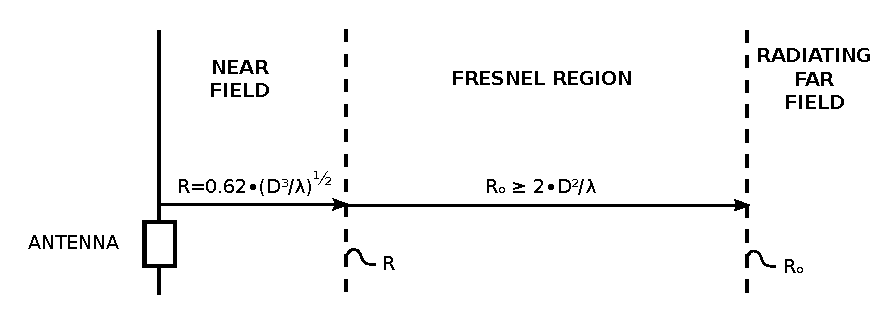
\includegraphics[width=0.9\textwidth]{./figs/02-state-of-the-art/FarNearFields-USP-4998112.pdf}
    \caption{Field for antennas larger than the wavelength of the radiation it emits~\cite{zerodamageFarFieldsVectorized1991}} 
    \label{fig:fieldregionsbigantenna}
\end{figure}

For small antennas, shorter than half of the wavelength of the emitting radiation, the \emph{near-field} for \ac{rfid} applications is usually upper limited by $\lambda / 2\pi = 0.159\lambda$~\cite{nikitinOverviewFieldUHF2007a}.
Small antennas are used in \ac{lf} and \ac{hf} \ac{rfid} technologies.
For these technologies, which depend on the \emph{near-field} for mutual coupling, the limit of the reactive region is theoretical limit for the read distance.
A delimitation of field regions for small antennas can be seen in figure~\ref{fig:fieldregionsshortantenna}.

\begin{figure}[!ht]
    \centering
    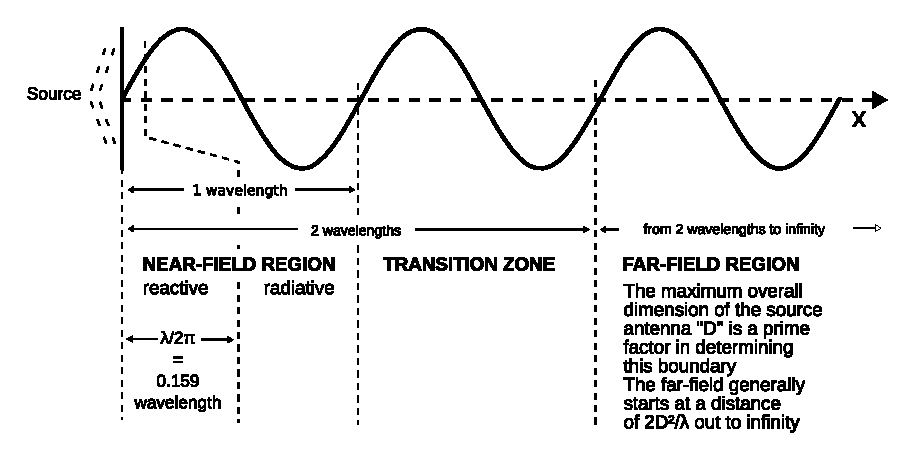
\includegraphics[width=0.9\textwidth]{./figs/02-state-of-the-art/Field_regions_for_typical_antennas_vector.pdf}
    \caption{Fields for antennas equal to, or shorter than, one-half wavelength of the radiation they emit~\cite{SafetyHealthTopics}} 
    \label{fig:fieldregionsshortantenna}
\end{figure}

\section{Tag} \label{sec:tag}

An \ac{rfid} tag is a device that can store and transmit data to a compatible reader in a contactless manner using radio waves or electro-magnetic fields.

Tag cost is the main factor in long term return on investment in \ac{rfid} systems. It is the most important consideration when designing systems. After the initial investment in infrastructure, the expenses are mainly the acquirement of new tags.
The reduction of cost per tag is the central focus of manufacturers and what allows the technology to be competitive in the world of \ac{scm}.

At its simplest composition~\footnote{an inductive RC resonant tag used in anti-theft systems is considered an \ac{rfid} device, but is far from the requirements of modern \ac{rfid} paradigms}, a tag contains a microchip and an antenna.
Depending on the technology the tag architecture and operation varies.
Tags are characterized by their chip, power source, memory characteristics and operating frequency. The following subsections will discussed these in detail.

\begin{figure}[!ht]
    \centering
    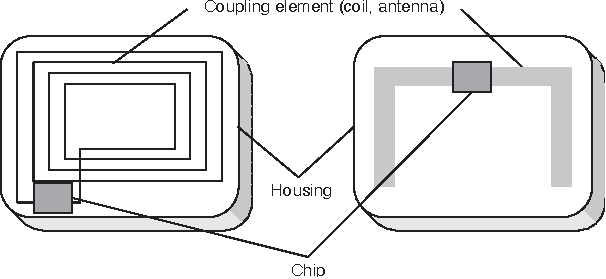
\includegraphics[width=0.65\textwidth]{./figs/02-state-of-the-art/tag.pdf}
    \caption{Components of a passive tag~\cite{finkenzellerRFIDHandbookFundamentals2003}} 
    \label{fig:passivetag}
\end{figure}

\subsection{Data Quantities}

In the contextualization of \ac{rfid} technologies presented in section~\ref{sec:contextualization}, we discussed the concept of identification and how it can be as simple as World War II \ac{iff} systems. 
An unidentified aircraft presents, upon radar lightening, its identification as being friend or foe. In computing language this can be abstracted as true or false, or $1$ or $0$. This kind of systems does not exchange more than a bit of information, the smallest unit of information, that can represent only two states.
This type of transponders are called $1$-bit transponders. Despite the limitations, they are still widely used in surveillance and and anti-theft systems. Apparel retailers and other goods retailers have been using them for almost $6$ decades and are still well established nowadays. 
This dissertation requires the identification of more than $2$ types of objects, so the following content will jump over technical explanations of this type of transponder~\cite{finkenzellerRFIDHandbookFundamentals2003}. 

The type of transponder discussed through out this dissertation are n-bit transponders which use an electronic microchip as the data carrying device.
These transponders can transfer data in different methods and are currently used in a variety of standards all over the globe.

The following sections of this chapter will approach concepts that are required to understand systems using n-bit tags, specifically \ac{uhfrfid}.
For a deeper analysis of other \ac{rfid} systems refer to \emph{The RFID Handbook by Klaus Finkenzeller}.

\subsection{Power Supply}

\subsubsection{Passive}

Passive tags are characterized for not having an on-board power source. 
Instead they use the power emitted from the reader antenna to energize itself and transmit the stored data to the reader.
As such, tag-to-reader communication is always started by a reader, since it needs to energize the tag.

This makes tags simple and cheap to manufacture, a microchip and an antenna is all there is to it. A few examples of state of the art passive \ac{uhf} tag inlays can be seen in figure~\ref{fig:alienAlienProductFamily2020}.
The simple constitution makes these tags robust, capable of withstanding corrosive chemicals such as acid and high temperatures~\footnote{The new Impinj M730 and M750 \ac{uhf} regular tags for item tagging sustains \ang{206}C for 1 minute and can retain data at \ang{125}C for 1 year~\cite[Tab. 18]{ImpinjM730M750}}.
These are the type of tags that underwent most technology advancements in the last decade in order to meet performance, compatibility and cost expectations that make mass deployment feasible for companies.

\begin{figure}[!ht]
    \centering
    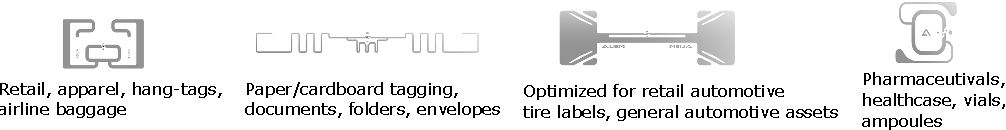
\includegraphics[width=\textwidth]{./figs/02-state-of-the-art/tag_examples.pdf}
    \caption{Selection of passive \ac{uhf} tag inlays for distinct applications from \textit{Alien Technology, LLC} 2020 Product Family~\cite{alienAlienProductFamily2020}} 
    \label{fig:alienAlienProductFamily2020}
\end{figure}

\subsubsection{Active}

Active tags have on-board power source and use it to transmit data to the reader.
These type of tags do not need reader's emitted power for data transmission, therefore, in tag-to-reader communication, tags can either communicate first or be interrogated by a reader.
Usually, active tags stay in a low-power state (i.e.\ sleep) in the absence of interrogation by the reader. When a reader wants to interact with a tag, issues a wake up command. The tag transits out the low-power state and resolves the interrogation.
The \ac{rf} environment generated by systems with these type of tags has generally much lower \ac{rf} noise.

Since the presence of the reader is not necessary for data transmission, an active tag can broadcast its data, like a beacon, to its surrounding even in the absence of a reader. This is what is denominated as \emph{transmitter}.
Widely used for \ac{iot} applications as \textit{wireless computers} to measure, process and transmit information about sensors, but out the scope of this dissertation. 

\begin{figure}[!ht]
    \centering
    \begin{subfigure}{.4\textwidth}
        \centering
        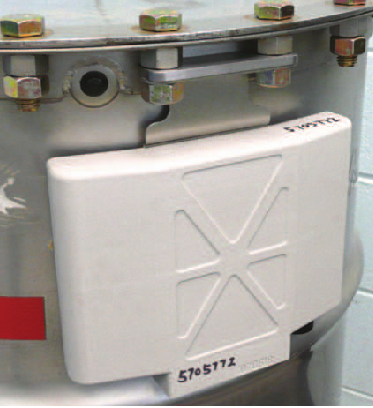
\includegraphics[width=.8\linewidth]{./figs/02-state-of-the-art/active_tag1.pdf}
        \caption{Tag mounted on Model 9975 drum}
        \label{fig:activetagsub1}
    \end{subfigure}
    \begin{subfigure}{.4\textwidth}
        \centering
        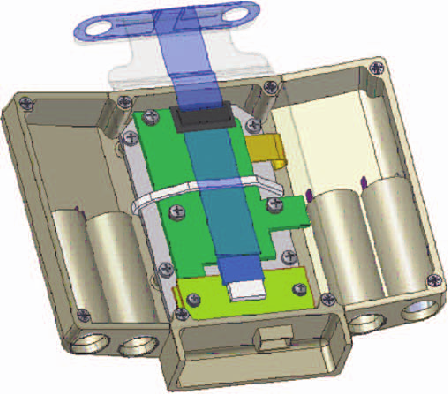
\includegraphics[width=0.95\linewidth]{./figs/02-state-of-the-art/active_tag2.pdf}
        \caption{Interior view of tag with metal back plate removed}
        \label{fig:activetagsub2}
    \end{subfigure}
    % Change caption
    \caption{\ac{us} Department of Energy prototype active tag with sensors for nuclear materials management working in $433.9MHz$ \ac{uhf} ISO band~\cite{tsaiApplyingRFIDTechnology2008}} 
    \label{fig:activetag}
\end{figure}

\subsubsection{Semi-passive}

Semi-passive tags, also called \emph{semi-active} or \emph{battery assisted} tag, have on-board power source but contrarily to active tags, it is only used for energizing the tag, thus, for transmitting its data, a semi-passive tag uses the reader's emitting power.

There are advantages of using these type of tags over passive ones.
Semi-passive tags do not use the reader signal to excite itself, so it can be read from further distances compared to passive tags. Because no time is needed to energize a semi-passive tag, it can also be read much faster than a passive one, making them useful for applications were the tag is in the reading zone for a short period of time (e.g.\ tolls on highways). Finally, this type of tag might also offer better readability in \ac{rf}-opaque and \ac{rf}-absorbent materials.

\begin{figure}[!ht]
    \centering
    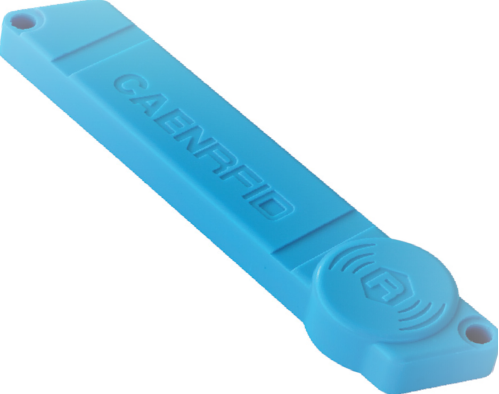
\includegraphics[width=0.3\textwidth]{./figs/02-state-of-the-art/semiactive_tag.pdf}
    \caption{\textit{CAEN RFID} A927Z semi-passive \ac{uhf} logger tag for temperature monitoring of sensitive products during transportation and storage~\cite{caenCaenA927ZTemp}} 
    \label{fig:semipassivetag}
\end{figure}

\subsection{Coupling}

We discussed in section~\ref{sec:em} how \acl{em} fields behave throughout the space surrounding a transmitting antenna. Lets now understand how \ac{rfid} technologies take advantage of \acl{rf} to establish a communication channel between reader and tag.

Coupling in \ac{rfid} refers to the energy absorbed by a receiving antenna when a transmitting one is operating. 
It is a fundamental concept in \ac{rfid} communications and affects several aspects of a system including range, frequency and cost.
The coupling method and operating frequency are the defining parameters of technology categorization in \ac{rfid}, presented in section~\ref{sec:opfrequency} and used all over the world as a baseline to describe \ac{rfid} systems.

There are three types of coupling techniques: inductive, capacitive and backscatter. 
This dissertation focuses on passive tag systems operating in the \emph{remote-couple} (i.e.\ range from $1$cm to $100$cm) and \emph{long-range} (i.e further than $100$cm).
Capacitive coupling is only exploited for data transmission in \emph{close coupling systems} (i.e.\ range less than $1$cm), therefore this type of coupling technique will not be discussed.

\subsubsection{Inductive}

Inductive-coupling systems, also known as magnetic-coupling, use the \emph{near-field} magnetic component of the \ac{emf} to establish a mutual coupling between reader and tag.

The reader antenna coil generates a strong high frequency \ac{em} field. The variation of the magnetic flux excites the cross-section of the tag coil and induces a voltage.
Considering the wavelength of the frequency range used (< 135 kHz: 2400m, 13.58MHz: 22.1m) is several times greater than the distance between reader antenna and the transponder, we can treat it just like a simple inductive coupling system, just like a transformer.

This voltage is rectified and supplied to the tag circuitry.
The circuitry is actually design to resonate at the transmission frequency of the reader. The resonance will generate high current in the reader, which produces the required field strength necessary for operation.

To transmit data from tag to reader, inductive systems use load modulation. The microchip changes de load on its coil in relation with the digital data to transmit. When a transponder, resonant at the transmission frequency of the reader, is placed in the reactive \emph{near-field} region, through mutual coupling, energy is drawn by the transponder, being detected by the reader as a voltage drop in the internal resistance of the reader through supply of current to the reader antenna.

\begin{figure}[!ht]
    \centering
    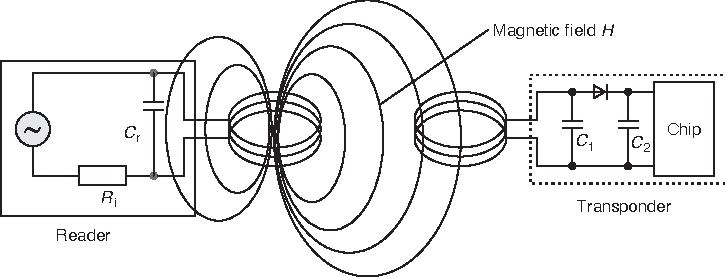
\includegraphics[width=0.9\textwidth]{./figs/02-state-of-the-art/loadmodulation.pdf}
    % Change caption
    \caption{Inductive coupled \ac{rfid} system overview~\cite{finkenzellerRFIDHandbookFundamentals2003}} 
    \label{fig:loadmodulation}
\end{figure}

This modulation method presents a fundamental problem. Due to weak coupling between antennas, there are voltage fluctuations at the antenna of the reader that are much higher than the fluctuations generated by the load modulation in the transceiver. This is a problem that usually appears in \ac{lf} \ac{rfid} systems. Detecting this slight voltages requires highly complicated circuitry which is undesirable.
Modern systems (e.g. $13.58$MHz \ac{hf} \ac{rfid}) use what is called: \emph{load modulation with subcarrier}. It uses the side bands created around the operating frequency ($f_T$) for the transmission of data. Switching the load resistor at a high elementary frequency ($f_s$), generates two spectral lines at a distance of $\pm f_s$ which contains the modulated signal. An illustration of this can be seen in figure~\ref{fig:loadmodulationsidebands}. The reader can demodulate and retrieve information that is carried in the sidebands of the two subcarrier sidebands, which are themselves created by the modulation of the subcarrier.

\begin{figure}[!ht]
    \centering
    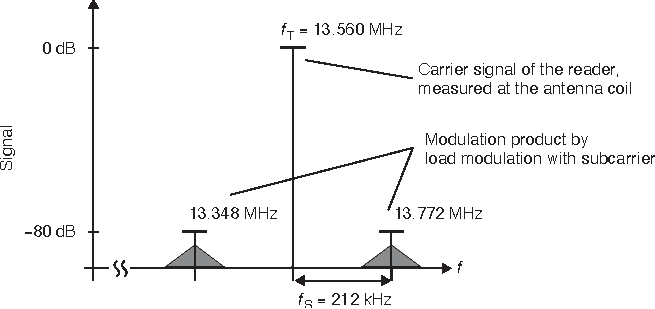
\includegraphics[width=0.7\textwidth]{./figs/02-state-of-the-art/loadmodulation_sidebands.pdf}
    \caption{Load modulation with subcarriers of a typical \ac{hf} \ac{rfid} system~\cite{finkenzellerRFIDHandbookFundamentals2003}} 
    \label{fig:loadmodulationsidebands}
\end{figure}

Despite wide scale use and established global standardization, this type of coupling presents a few drawbacks. The reading distance is physically limited by the size of the reader antenna and the reactive \emph{near-field} boundary discussed through out section~\ref{sec:em}. The shrinkage of tag size is technically challenging due to the power emissions regulations and the dependence with the variation of the magnetic flux through the cross-section of the tag antenna coil that excites the tag circuitry. The power consumption is also much higher than the next coupling technique we will look at, making it unsuitable for \emph{long-range systems}.

\subsubsection{Backscatter}

Backscatter coupling harvests energy from the \ac{emw}, transmitted by the reader antenna, to power the tag circuitry. It is mainly used in \emph{long-range systems} since it is the primarily coupling technique capable of operate in the \emph{far-field} region.
To transmit data back to the reader, the tag \textit{reflects} back some of the power as a modulated signal through what is called \emph{modulated reflection cross-section}.

\emph{Modulated reflection cross-section} functions by the same fundamental principles as the first \ac{rfid} system invented, presented in section~\ref{sec:contextualization}.
\ac{emw} are reflected by objects with dimensions greater than around half the wavelength of the wave.
The efficiency with which an object reflects \ac{emw} is described by its \emph{reflection cross-section}. Objects that are in resonance with the wave front that hits them, as is the case for antennas tuned to the appropriate frequency, have a particularly large \emph{reflection cross-section}.

The modulation of the \ac{rf} signal is created by changing the impedance viewed from the tag antenna, in similar manner to inductive coupling systems. 
Depicted in figure~\ref{fig:backscatter}, a load resistor, connected in parallel with the antenna, is switched on and off in time with the data stream to be transmitted.
The power reflected back changes in amplitude with the changing of impedance of the tag.
The reflected signal is picked by the reader antenna. decoupled using a \emph{directional coupler} and demodulated~\cite{finkenzellerRFIDHandbookFundamentals2003, RFIDCouplingTechniques}.

\begin{figure}[!ht]
    \centering
    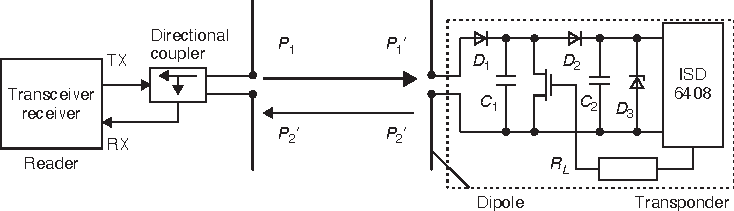
\includegraphics[width=0.9\textwidth]{./figs/02-state-of-the-art/backscatter.pdf}
    \caption{Passive backscatter RFID system~\cite{finkenzellerRFIDHandbookFundamentals2003}} 
    \label{fig:backscatter}
\end{figure}

\subsection{Technologies} \label{sec:opfrequency}

When categorizing systems, the main aspect that defines \ac{rfid} technologies is the operating frequency.
In the previous sections we noticed a clear relation between operating frequency, through the wavelength, and system specifications like reading distance and data transfer speeds.
So, it is no accident that this spontaneous categorization happened. \ac{rfid} technologies tend to mature in a very clear path, being encompassed under use case specific standards with fixed operating frequencies carefully assigned by regulatory \ac{rf} authorities in each country. 
It is indeed a useful classification method to summarize a set of specifications that usually need to established a priori to system design.

Being so, it is common in \ac{rfid} slang to name systems by the frequency band they operate in.
There are five preeminent frequency groups: \ac{lf}, \ac{hf}, \ac{uhf}, Microwave and \ac{uwb} which will not further discussed being in early phases of technological development.
Each of the frequency groups presents characteristics inherent to their physical limitations that should be considered when choosing a technology.

\paragraph*{\ac{lf}} usually operate in the $125$KHz to $134$KHz frequency range, using passive tags through inductive coupling. Inherently, it has slow read speed and the reading range is limited to around $0.5m$. Despite the drawbacks, they have good behavior in metals and liquids and are the most mature technology, probably having the largest installed based system.
It is widely used in animal identification (ISO 11784/5~\cite{isoISO117841996, isoISO117851996}, ISO 14223~\cite{isoISO1422332018}), access control, logistics and data collection~\cite{isoISOIEC180002} and automotive industry in car ignition keys, to say a few.

\paragraph*{\ac{hf}} operates mostly around the $13.54$MHz frequency band. In same manner as \ac{lf}, it uses inductive coupling. The higher operating frequency allows faster data read speeds while maintaining semi-decent behavior in metals and liquids.
Widely used in smart cards~\cite{isoISOIEC156932, MIFARE} for all kinds of applications and is the basis of \ac{nfc} technology~\cite{isoISOIEC144434, isoISOIEC180003}. \ac{nfc} has been receiving a lot of attention. It is a global communication standard with a mature market (being in ruffly any smartphone nowadays). This convened big companies to invest in it, which promoted wide scale manufacturing, resulting in the reduction of tag price (\$0.35 - \$10.00 per tag) and increase in system deployments.

\paragraph*{\ac{uhf}} operates in the band of $315$MHz to $433$MHz using active tags~\cite{isoISOIEC180007}, and in $860$MHz to $956$MHz using passive ones~\cite{isoISOIEC180006}. It is known for the promises it brings to \ac{scm} and logistics, being a cheap and affordable technology to wirelessly identify and track every item. It is mainly used in item tracking but it can be used for all kinds of applications. It uses backscatter coupling to transmit data between reader and tag. These frequencies present some drawbacks: poor behavior on liquid and metals is a big problem with passive tags; the allocation of the \ac{rf} spectrum differs between countries being a huge problem for global deployments. This thematic will be further discussed throughout this dissertation.

\paragraph*{Microwave} typically operates at $2.45$GHz~\footnote{$5.8$GHz ISO standard was withdrawn}~\cite{isoISOIEC180004} which is also called \emph{Industry, Scientific, and Medical (ISM)} band, accepted globally. Uses backscatter coupling with passive, semi-passive and active tags. It performs very poorly in the presence of metals and liquids. 

For concise information related to each band, consult table~\ref{tab:rfproperties} for \ac{rf} properties in different materials and tables~\ref{tab:} for an abridgment of much general information.

\begin{table}[!htb]
    \centering
    \caption{\ac{rf} properties in different materials~\cite{lahiriRFIDSourcebook2005}}
    \begin{tabular}{|l|l|l|l|l|}
    \hline
    \textbf{Material}     & \textbf{LF} & \textbf{HF} & \textbf{UHF} & \textbf{Microwave} \\ \hline
    Clothing              & RF-lucent   & RF-lucent   & RF-lucent    & RF-lucent          \\ \hline
    Dry wood              & RF-lucent   & RF-lucent   & RF-lucent    & RF-absorbent       \\ \hline
    Graphite              & RF-lucent   & RF-lucent   & RF-opaque    & RF-opaque          \\ \hline
    Liquids (some types)  & RF-lucent   & RF-lucent   & RF-absorbent & RF-absorbent       \\ \hline
    Metals                & RF-lucent   & RF-lucent   & RF-opaque    & RF-opaque          \\ \hline
    Motor oil             & RF-lucent   & RF-lucent   & RF-lucent    & RF-lucent          \\ \hline
    Paper products        & RF-lucent   & RF-lucent   & RF-lucent    & RF-lucent          \\ \hline
    Plastics (some types) & RF-lucent   & RF-lucent   & RF-lucent    & RF-lucent          \\ \hline
    Shampoo               & RF-lucent   & RF-lucent   & RF-absorbent & RF-absorbent       \\ \hline
    Water                 & RF-lucent   & RF-lucent   & RF-absorbent & RF-absorbent       \\ \hline
    Wet wood              & RF-lucent   & RF-lucent   & RF-absorbent & RF-absorbent       \\ \hline
    \end{tabular}
    \label{tab:rfproperties}
\end{table}

\begin{landscape}
    \begin{table}[]
        \begin{tabular}{@{}lllllll@{}}
        \toprule
        \textbf{Name} & Frequencies                                                                   & Coupling                                                         & Range           & Protocols                                                                                     & Price                                                                       & Disadvantages                                                                     \\ \midrule
        LF            & 125 - 135 KHz                                                                 & \begin{tabular}[c]{@{}l@{}}Inductive, \\ Capacitive\end{tabular} & \textless 0.5 m & \begin{tabular}[c]{@{}l@{}}Animal ID,\\ factory data collection\end{tabular}                  & US\$1                                                                       & \begin{tabular}[c]{@{}l@{}}Short reading range,\\ Slow reading speed\end{tabular} \\
        HF            & 13.553 - 13.567 MHz                                                           & \begin{tabular}[c]{@{}l@{}}Inductive,\\ Capacitive\end{tabular}  & \textless 1 m   & \begin{tabular}[c]{@{}l@{}}Smart cards (ISO/IEC 15693, ISO/IEC 14443 A, B)\\ ...\end{tabular} & US\$0.50 to US\$5                                                             &                                                                                   \\
        UHF           & \begin{tabular}[c]{@{}l@{}}433 MHz, \\ 858-960 MHz\end{tabular}               & Backscatter                                                      & \textless 9 m   & ...                                                                                           & \begin{tabular}[c]{@{}l@{}}US\$5 (active), \\ US\$0.15 (passive)\end{tabular} &                                                                                   \\
        Microwave     & \begin{tabular}[c]{@{}l@{}}2.4 - 2.454 GHz, \\ 5.725 - 5.875 GHz\end{tabular} & Backscatter                                                      & \textless 10 m  & ...                                                                                           & US\$5 projected                                                             &                                                                                   \\ \bottomrule
        \end{tabular}
    \end{table}
\end{landscape}

\section{Reader} \label{sec:reader}

A reader is a device that can read from and write data to compatible \ac{rfid} tags. It is responsible for sending and receiving \ac{rf} signals to and from tags.
If we strip down all the features modern readers offer, we can isolate three main components: \ac{rf} front-end, processor, communication interface.

The \ac{rf} front-end interfaces with the reader antenna. 
It is responsible for transmitting power and clock cycle via the antenna to tags in the reading zone, and demodulate \ac{rf} signals received from tags to be further handled by the processor. 
Readers must adhere to \ac{rf} modulation requirements and \ac{eirp} regulations if they want to be approved and commercialized. This fact promotes the implementation of the front-end by a dedicated transceiver microchip and complementary electronics, which is usually chosen. There are also efforts in implementing the \ac{rf} front-end in \acp{fpga}, which might change this paradigm in the next few years~\cite{hugomanueloliveirademirandaSistemasRFIDUHF2015}.

The processor is responsible for all logic necessary in the reader. It often comes with other complementary components like memory and dedicated \acp{ic} for specific tasks. Readers differ in architecture design between manufacturers, but the processor must at least implement the reader protocol to communicate with compatible tags. This includes decoding and error checking of the analog signals from the \ac{rf} front-end, a controller interface to allow external entities to communicate with it, to transfer stored data, issue commands, accept commands and control the reader functions.

Communication interface is the component that provides communication instruction to a reader which allows external entities to interact with it.
It usually comes inside microprocessors and microcontrollers \acp{ic}. It usually seen in commercial readers as serial communication interface or ethernet.

Commercial readers come a variety of types which are suited for different applications.
The most common are stationary readers. Also called, \emph{fixed} readers, they are what the name implies, used for making fixed reading zones. They also can be mounted on forklifts and inside of trucks.
Other types are handheld readers, for a portable reading device and \ac{rfid} printers which are used to print smart labels.

\section{Reader Antenna} \label{sec:antenna}

A reader communicates with tags through its antenna. 
Antennas are responsible for converting guided \acp{cw} in radiating \ac{emw} and vice-versa.
It will only be covered radiating antenna theory for it is what is necessary to follow this dissertation.

In handheld readers, the antenna is generally integrated in to the device. In stationary readers is most commonly found as a separate device attached to an antenna port of the reader by means of a cable.
There are different groups of antenna designs: antennas composed of a wire, which encompass the dipole, monopole and loop antennas; constituted of an opening, like the horn and cavity backed slot antennas; and printed circuit antennas like path antennas, commonly used in \ac{uhfrfid}.

Evaluating antennas for \ac{rfid} systems can be done through the parameters specified by the manufacturer, a few rules of thumb and engineering sensibility.
At \ac{uhf} we can control the direction of waves and other parameters, and thus improve the readability of tags.

\subsection{Radiation pattern}

An important parameter in antenna selection is the radiation pattern. 
Radiation pattern is the mathematical description or representation of the radiation properties of the antenna as a function of space coordinates.
It illustrates the regions where the antenna's energy is most effective.
In \ac{rfid} is usually called the footprint of the antenna and determines the read zone.
Manufacturers usually provide the radiation patterns for \ac{rfid} antennas in the datasheet.

Different antenna designs radiate different patterns. These radiation patterns are classified in three main classes: isotropic, directional and omnidirectional.
For \ac{uhfrfid}, directional antennas are really useful since it is possible o maximize directivity, that is, how well the radiation emitted is concentrated in a single direction. This increases reading distances and defines boundaries in reading zones. \ac{uhfrfid} directional antennas are commonly patch antennas, also called \emph{microstrip} or \emph{planar antennas}. They consist of rectangular metal foil or a plate mounted on a substrate such as Teflon or FR-4 (i.e.\ woven fiberglass cloth with an epoxy resin binder).

Is also important, when designing \ac{rfid} systems, to have notion of the deformations that occur in the radiation patterns.
\emph{Multi-path} phenomena - the reflection of \ac{emw} in \ac{rf}-opaque objects which causes waves to be scattered and arrive back at the reader in different paths and times - results in \emph{phase} shifts as constructive and destructive interference.
This creates protrusions and dead zones that will inevitably exist in most \ac{uhfrfid} and microwave systems deployments. 

%\subsection{Gain}

%They gain parameter is also "important" when selecting an \ac{rfid} antenna.
%It characterizes the performance of the antenna by mathematically describing how well it converts input power into radio waves radiated in a specified direction. It relates directivity and efficiency.

\subsection{Polarization}

Antennas radiate \ac{emw} into surrounding space.
Polarization is the direction of oscillation of the \ac{emw} and has a great importance in tag readability.

\acp{emw} behave similarly to a wave of water. When a wave from a source, like a boat, reaches a buoy, the buoy moves mostly up and down.
Analogously, \ac{emw} moves electrons in the plane perpendicular to the direction of propagation. The direction in which the field points, determines the polarization of the \ac{emw}.
Unlike water waves, \acp{emw} are not influenced by gravity, so the electric field can point in any direction in the plane perpendicular to the direction of propagation, and so have different polarizations~\cite{dobkinRFRFIDSecond2012}.

The main types of polarization are known as linear and circular. Both types derive from the elliptical polarization, being linear and circular special cases of such.

\subsubsection{Linear polarization}

Linear polarized antenna emanate \acp{emw} in a linear pattern, that is, emits \ac{emw} with only one field of energy.

These antennas have a narrower radiation beam with better directivity compared to circular polarized antennas. This results in longer reading distances and well-defined reading regions, which are essential to good \ac{rfid} system design.

These advantages can sometimes fall short to the disadvantages. Linear antennas are sensitive to tag orientation with respect to its polarization direction. 
\ac{rfid} tag antennas are usually dipoles constituted of narrow metal traces aligned in one direction. If the electric field is directed along the traces, it can push electrons back and forth inducing the voltage necessary to energize the tag \ac{ic}. If the electric field is directed perpendicular to the trace axis, it moves electrons across the diameter of the trance, producing negligible current, insufficient to power the tag \ac{ic}.
Linear antennas are generally used in applications where tag orientation is fixed and predictable, or in conjunction with other complementary linear antennas.

\subsubsection{Circular polarization}

Circular polarized antennas solve, to certain degree, the orientation dependence problem with detriment of reading distance and a wider radiation beam.
These antennas have two constituting energy fields that are equal in amplitude and magnitude, with a phase difference of $90^\circ$ between them. This results in the electric field vector to be seen as helix like trace, a circular motion propagating through space. 

Because the nature of circular polarized antennas, they are to a certain extent, unaffected by tag orientation.
A circularly polarized \ac{emw} interacts with the linear antenna of a tag, tilted at any angle within the plane perpendicular to the axis of propagation, but in every case only half the transmitted power can be received.
Good antenna design in tags can modestly improve energy harvesting performance, e.g.\ incorporate two dipole antennas on the tag directed orthogonally to one another or physically larger bow-tie antenna designs.

These antennas are widely used in passive \ac{uhfrfid}, specially in \ac{rf} environment with high degree of \ac{rf} reflectance, like due to presence of metals.

\cleardoublepage
%\chapter{EPCglobal Architecture Framework} \label{sec:epcglobal}

\section{Context}

Advances in \acs{uhf}~\acs{rfid} gathered a lot of attention and investment in the beginning of the decade. The technology promised, for years, a disruption in the \ac{scm} which was never delivered. 

Item level identification allows companies to capture product lifecycle information at remarkable levels of detail. \ac{rfid} readers placed through out the supply chain can automatically capture information about tagged objects while they move from manufactured to consumer.
An infrastructure that bridges the gap between the physical and the digital world, providing real-time information about current supply chain operations.
Furthermore, the instant share of information between intervening companies increases supply chain visibility, resulting in reduced uncertainty in operational and tactical supply chain planning.
Stock levels could be precisely controlled and shared with trading partners, which in turn reduces inventory costs and optimizes intra-company operations~\cite{lorenzDiscoveryServicesEPC2011, simchi-leviCadeiasSuprimentosProjeto2003}.

It was an utopia ahead of its time. The technology was not mature enough, the return on investment was not appealing and cloud computing had just started to get traction.

This did not stop the conceptualization and development of architectures capable of delivering the promises we were hoping for.
The architecture that stood relevant through out these uncertain times is the \emph{EPCglobal Architecture Framework}.
It was created and maintained by GS1, a non profit organization tasked with developing global standards for business communications.
The organization has the experience, resources and influence to make this utopia a reality.
The architecture shows on paper an appealing concept of a network capable of doing amazing thing for the \ac{scm} without restricting businesses \ac{it} architectures.

\subsection{Standardization Efforts}

Standardization of \acs{uhf}~\acs{rfid} for item level tagging and supply chain, by organizations like GS1, provided a common language to identify, capture and share supply chain data, ensuring important information is accessible, accurate and easy to understand~\cite{anonymousStandardsGS12014}.

The first prominent adoption was by the \ac{us} \ac{dod} with a policy released on July 30th 2004. The policy stated that contracts issued for material delivery would require the use of \ac{uhf} tags. The policy was later extended to all commodities and commodities pallets shipped to any \ac{dod} facility~\cite{DoDSuppliersPassive, DODReleasesFinal}.

In 2014, Impinj, Intel, Google and Smartrac, joined forces to create the RAIN RFID alliance after the ratification of GS1's \acs{uhf}~\acs{rfid} Generation 2 version 2 standard in November of 2013. The alliance promotes the universal adoption of GS1's Gen2 \acs{uhf}~\acs{rfid} technologies and cloud computing, where \ac{rfid}-based data can be stored, managed and shared via the Internet~\cite{WhatRAINRFID}.
The alliance fortified the adoption of GS1's standards and traced a common path for the industry to progress~\cite{TechnologyCompaniesCreate}.

On October 11th 2018 the European Commission published their positive implementation of the upper band for European countries~\cite{302208v030101pPdf}.
It extended the power levels to $2W$ in the lower band and added the requested global band from $915$MHz to $921$MHz with power levels up to $4W$. 
This was the biggest effort by the European Commission to establish a global standardized frequency band for \acs{uhf}~\acs{rfid} supply chain applications.

\subsection{Current Problems} \label{sec:currentproblems}

There are still \ac{rfid} tags that do not conform with the international standards, often presenting proprietary formats and even encoding errors.
These closed practices and struggle for market supremacy around \acs{uhf}~\acs{rfid} creates a problematic situation that prevents conformity through the global logistics market.

Even in global standards, the adoption depends on the company and field of business. Usually one identification standard is already being used, and the migration cost for supporting multi-code integration can be high.

The information around global standards is also limited and hard to get through. It is divided in multiple specifications, identified with number notation and codification nomenclature. 
The ISO standards, in specific, are closed and have to be payed before even see its contents.
These specifications are extensive and don't provide newcomers a good experience. 
Companies planning to implement \acs{uhf}~\acs{rfid} systems following legitimate global standardization resort to consultants who have a deep knowledge on the standards complexity.

The closed mentality in the area slowed the industry progression. In comparison with the cloud and web industries, where experience and software is shared and open-sourced, \acs{uhf}~\acs{rfid} tends to keep everything closed~\cite{WhatCouldSlow}. The existent freely available software is old, outdated and out of maintenance. Experience from real-world implementations is unavailable and it is not shared, making the industry prone to committing recurrent mistakes. This results in high investments in time and money on engineering resources that could be shared among industry leaders.

The positive implementation of the upper band frequency in Europe for global \acs{uhf}~\acs{rfid} supply chain applications is also dependent on the acceptance by each European members. In particular, Germany and Netherlands are not accepting it~\cite{EUUpperBand}. The conflict with existing adopted bands in the countries makes a global homogeneous system a challenge that will need time to be established.

\subsection{GS1 and EPCglobal}

GS1 is a nonprofit organization dedicated to the development and implementation of standards for global supply chain solutions. 
The institution mission is to manage the GS1 System of Standards, create open, global, multi-sector standards fostering good business practices.

GS1 established itself in 2005 from the \ac{ean} International, \ac{ucc} and other local organizations from the United States~\cite{PublicationLEBENSMITTELZEITUNGa}.
The organization took under its umbrella the former \acs{ean}-\acs{ucc} roles subsuming their technologies. From those technologies, it is worth mentioning: the barcode identification system (from \ac{ean}), \ac{xml} standards, \ac{edi} transaction sets and supply chain solutions~\cite{lahiriRFIDSourcebook2005}.

The new GS1 organization then adopted much more ambitious projects, developing global standards and services for business communication.
From those efforts resulted the network for the synchronization of master data \ac{gdsn}, the \ac{epc} integration for \ac{rfid}, traceability and the upstream integration of the consumer goods industry suppliers and \emph{EPCglobal Network}.

For RFID Technology to become viable in practice, an infrastructure must exist for processing and communicating EPC data. In meeting the goal of creating a common infrastructure, \ac{mit} announced Auto-ID Release $1.0$ in October 2003. At the same time, \ac{mit} entered into an exclusive licensing agreement with GS1.
In turn, GS1 established a new division called EPCglobal to implement Release $1.0$ and to conduct further development based on industry input. This put forth an initial set of standards that formed the infrastructure for \ac{epc} data. Later, Auto-ID Release $1.0$ became the starting-point for the \emph{EPCglobal Network} and Architecture Framework~\cite{GlobalRFIDValue}.

\section{Overview}
%Activities, Standards, Goals

%EPC Uniqueness, Identifiers, Decentralized Implementation, Issuing Organization
%Review text - it is from and ex subsection prior to the revision of the new index

\emph{EPCglobal Architecture Framework} is a collection of interrelated hardware, software, and data standards that interoperate with shared network services~\cite{GS1EPCglobalArchitecture}.
These services are referred to as \emph{EPCglobal Network}, a computer network used to share \ac{epc} data between trading partners.
They are operated by GS1, its delegates and others to provide automatic, real-time identification and data sharing of items both within and outside of a company~\cite{lahiriRFIDSourcebook2005}.

The framework defines information systems, interface standards and data models. This approach frees the market of \ac{it} systems to create custom business solutions. Manufacturing can have their custom business logic closed, and expose production state information to the clients through the \emph{EPCglobal Network} with the EPCglobal interface standards.

The existence of these standards promote not only the global adoption of \ac{epc}, but also the exchange of information between business partners.
Even though the network was designed primarily for \ac{rfid} \ac{epc} data sharing, the network does not exclusively run on \ac{rfid} data carriers. The Network can also be fed \ac{epc} data through data carriers like 1D and 2D barcodes. The interoperability with the barcode was one of the most important considerations during the planning of the network~\cite{RFIDBarcodeInteroperability}.

\subsection{Activities} \label{sec:activities}

The architecture defines three core activities, all of which have a group of standards and guidelines within the \emph{EPCglobal Architecture Framework}: \emph{Physical Object Exchange}, \emph{Infrastructure for Data Capture} and \emph{Data Sharing}, which I will be briefly brainstorm bellow.
These activities are helpful in understanding the organization and scope of the framework but should not be interpreted as extremely rigid~\cite{GS1EPCglobalArchitecture}.

\subsubsection{Physical Object Exchange} 

\emph{Identify} individual physical objects - products, cases, loads, assets, return items, among others - so they can be tracked individually.
Entities in the supply chain exchange physical objects identified with \acp{epc}.
Exchange operations can be such as shipping, receiving goods, and so on.
For many End Users, the physical objects are trade goods, but this could not be the case.
There are many other use cases, like library or asset management applications~\cite{dong-yingliDesignInternetThings2016} that differ from the supply chain trade goods model, but still involve unique identification and tagging of objects. 
The architecture must be designed to ensure that when one \emph{End User} delivers a physical object to another end user, the latter will be able to determine the \ac{epc} of the physical object and interpret it properly~\cite{GS1EPCglobalArchitecture}.

\subsubsection{Infrastructure for Data Capture} 

\emph{Capture data} about the movement of physical assets to create supply chain visibility.
In order to gather \ac{epc} data, each \emph{End User} carries out operations within its environment. Those can be: the creation of \acp{epc} for new objects, follow the movements of objects by sensing their \acp{epc}; and gather that information into recording systems within the organization~\cite{GS1EPCglobalArchitecture}.

\subsubsection{Data Sharing} 

\emph{Exchange data} with \ac{it} applications and trading partners, to turn visibility into information and action.
\emph{End Users} benefit from the \emph{EPCglobal Architecture Framework} by sharing data with each other, increasing the visibility they have regarding movement of physical objects through the supply chain. 
The \emph{EPCglobal Architecture Framework} standards provide a means for \emph{End Users} to share data about \acp{epc} within defined user groups or the general public. 

% image: \emph{EPCglobal Architecture Framework} activities~\cite{Architecture6framework20140414Pdf}


\subsection{Brief}

% check EPCIS standard document section 2

% This standard defines EPC tag data formats for Generation 2 tags. It defines how the EPC is encoded on the tag and how it is encoded for use in the information systems layers of the EPC Systems Network. The standard includes specific encoding schemes for EPC General Identifier (GID).

The \emph{EPCGlobal Architecture Framework} can be difficult to analyse and use. It is separated in multiple specifications and shows inconsistencies between documents, making the introduction to the framework fairly hard.
Throughout this section I will introduce the baseline implementation of the \emph{EPCGlobal Architecture}, introducing each intervening member and their role within the framework. This brief searches to provide a technical contextualization of the architecture for the next sections, where it will be thoroughly explained.

The \emph{Architecture Framework} provides detailed specifications for three technologies developed by EPCGlobal: the \acf{epc}, components of the \emph{EPCGlobal Network™} and standards for \ac{rfid} readers and tags.

The \ac{epc} is a unique \acs{id} used to identify an object. This \ac{epc} can be stored in different physical formats, including in \ac{rfid} tags. 
These \ac{epc} enabled \ac{rfid} tags can be attached to objects, and inspected throughout the supply chain by a network connected by services and readers.
The simplest implementation of the \emph{EPCGlobal Framework} can be structured like shown in figure~\ref{fig:archstructure}.
I will start on the bottom and go up in the architecture structure.

\begin{figure}[!ht]
    \centering
    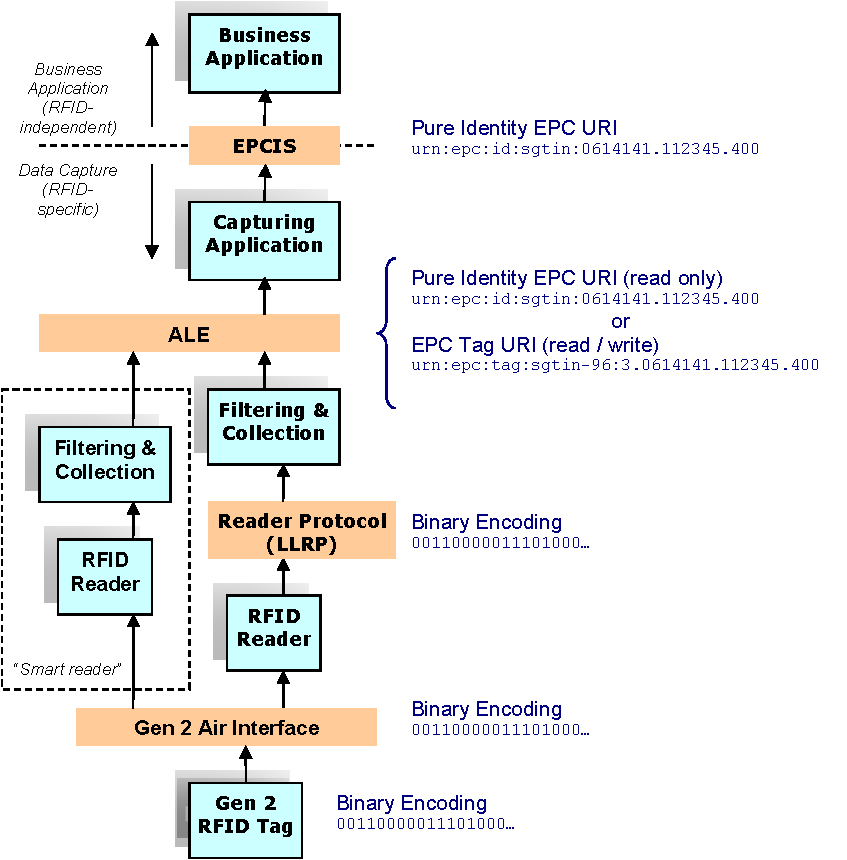
\includegraphics[width=\textwidth]{./figs/02-state-of-the-art/architecturer_structure.pdf}
    \caption[\emph{EPCGlobal Architecture Framework} baseline example with \ac{epc} representations used at each level]{\emph{EPCGlobal Architecture Framework} baseline example with \ac{epc} representations used at each level~\cite{EPCTagData}} 
    \label{fig:archstructure}
\end{figure}

The \ac{gen2} \ac{rfid} Tag is the latest generation of the \ac{uhf} tag standard design by EPCGlobal. \ac{gen2} tags communicate with readers through the \ac{gen2} Air Interface. The physical memory map of \ac{gen2} tags is standardized in the \ac{tds}~\cite{EPCTagData}, in conjunction with the binary encoding of \acp{epc}. The \ac{rf} communication link, signaling and commands between \ac{gen2} tags and readers is defined in the \ac{gen2} \ac{uhf} \ac{rfid} Standard~\cite{UHFGen2Tag}.

Readers communicate with clients through the \ac{llrp} standard~\cite{LowLevelReader}. \ac{gen2} readers can generate large amounts of network traffic and data, which needs to be processed. For that, \emph{EPCGlobal Architecture Framework} defines \acf{fc} middleware, to translate binary \acs{epc} into human readable format, and filter/aggregate data. \ac{fc} can be implemented in the same physical device as the reader, being called a ``smart reader''. 

Middlewares then send the processed data to Capture Applications, where \ac{epc} data is contextualized with business logic. Middlewares send this data through an \ac{ale} interface. The \ac{ale} interface allows Capture applications to register and subscribe to their interested \ac{epc} patterns and request strategies in a high-level declarative way. The interface is defined in its two documents~\cite{ApplicationLevelEvents} and \cite{ApplicationLevelEventsa}.

Capture Applications send the contextualized data to Business Applications or data repositories.
This data is sent following strict rules to ensure data is created and shared in a conformable and standardized way. The \emph{EPCGlobal Architecture Framework} defines the \ac{epcis}~\cite{EPCInformationServices} and \ac{cbv}~\cite{CoreBusinessVocabulary} Standards, containing data models, vocabulary and communication interfaces required to create and share \ac{epc} related data with trading partners.

More standards and information paradigms exist in the \emph{EPCGlobal Architecture Framework}, namely in the \emph{EPCGlobal Network™} group of standards. The standards under the authority of \emph{EPCGlobal Architecture Framework} can be seen in table~\ref{tab:standards}. Relevant standards and congruous paradigms not in the practical scope of this dissertation: \acf{rm} standard to manage readers (not strongly adopted by the community); \acf{dci}; \acf{tdt} for validation and translation of \ac{epc} identifiers; \ac{ons} a protocol to discover information about a product and related services from the \ac{epc}; and \acf{gdsn}, the network of interoperable data pools to share master data with their trading partners in a standard method. 

\begin{table}[]
    \begin{adjustwidth}{-0.09\textwidth}{0em}
    \begin{tabular}{|l|l|l|}
    \hline
    \textbf{Activity}                                                                       & \textbf{Standard}                                                                                                                                           & \textbf{Status}                                                                                                                                                                                                                \\ \hline
    Object Exchange                                                       & \emph{\acs{uhf} Gen 2 Tag Air Interface}                                                                                                          & Ratified Jul 2018 v2.1.0~\cite{UHFGen2Tag}                                                                                                                                                                        \\ \cline{2-3} 
                                                                                            & \acs{hf} Class 1 Tag Air Interface                                                                                                         & Ratified Sep 2011 v2.0.3~\cite{HFClassTag}                                                                                                                                                                        \\ \cline{2-3} 
                                                                                            & \emph{\acs{epc} Tag Data Standard (\acs{tds})}                                                                                               & Ratified Nov 2019 v1.13~\cite{EPCTagData}                                                                                                                                               \\ \cline{1-1}
    \begin{tabular}[c]{@{}l@{}}Data Capture \\ Infrastructure\end{tabular} &                                                                                                                                                             &                                                                                                                                                                                                                                \\ \cline{2-3} 
                                                                                            & \emph{Low Level Reader Protocol (\acs{llrp})}                                                                                                     & Ratified Oct 2010 v1.1~\cite{LowLevelReader}                                                                                                                                                             \\ \cline{2-3} 
                                                                                            & Reader Management (\acs{rm})                                                                                                               & Ratified May 2007 v1.0.1~\cite{ReaderManagementRM}                                                                                                                                                       \\ \cline{2-3} 
                                                                                            & \begin{tabular}[c]{@{}l@{}}Discovery, Configuration, and \\ Initialization (\acs{dci}) for Reader Operations\end{tabular}                  & Ratified Jun 2009 v1.0~\cite{DiscoveryConfigurationInitialization}                                                                                                                                       \\ \cline{2-3} 
                                                                                            & \emph{Tag Data Translation (\acs{tdt})}                                                                                                           & Ratified Oct 2011 v.1.6~\cite{tdtTagDataTranslation}                                                                                                                                                     \\ \cline{2-3} 
                                                                                            & \emph{Application Level Events (\acs{tds})}                                                                                                       & Ratified March 2009 v1.1.1~\cite{ApplicationLevelEvents, ApplicationLevelEventsa}                                                                                                                        \\ \cline{2-3} 
                                                                                            & \emph{\acs{epcis} Capture Interface}                                                                                                              & \acs{epcis} Ratified                                                                                                                                                                                                                 \\ \cline{2-3} 
                                                                                            & \begin{tabular}[c]{@{}l@{}}\emph{\acs{epcis} Data Standard}\\ \emph{Core Business Vocabulary (\acs{cbv})}\end{tabular} & \begin{tabular}[c]{@{}l@{}}\acs{epcis} Ratified Sep 2016 v1.2~\cite{InformationServicesEPCIS}\\ \acs{cbv} Ratified Oct 2017 v1.2.2~\cite{CoreBusinessVocabulary}\end{tabular} \\ \cline{1-1}
    Data Sharing                                                           &                                                                                                                                                             &                                                                                                                                                                                                                                \\ \cline{2-3} 
                                                                                            & \emph{\acs{epcis} Query Interface}                                                                                                                & \acs{epcis} Ratified Sep 2016 v1.2~\cite{InformationServicesEPCIS}                                                                                                                                             \\ \cline{2-3} 
                                                                                            & Pedigree Standard                                                                                                                                           & Ratified Jan 2007 v1.0~\cite{PedigreeStandardV1}                                                                                                                                                         \\ \cline{2-3} 
                                                                                            & EPCglobal Certificate Profile                                                                                                                               & Ratified Jun 2010 v2.0~\cite{EPCglobalCertificateProfile}                                                                                                                                                \\ \cline{2-3} 
                                                                                            & Object Name Service (\acs{ons})                                                                                                            & Ratified Jan 2013 v2.0.1 ~\cite{deanGS1ObjectName}                                                                                                                                                       \\ \cline{2-3} 
                                                                                            & Global Data Synchronisation Network (\acs{gdsn})                                                                                           & Ratified Nov 2020 v3.1.14~\cite{joe.horwoodGDSNStandardsMaintenance}                                                                                                                                     \\ \cline{2-3} 
                                                                                            & \begin{tabular}[c]{@{}l@{}}Lightweigh Verificationt Messaging \\ Standard\end{tabular}                                                                      & Ratified Jul 2019 v1.1~\cite{david.buckleyGS1LightweightVerification2019}                                                                                                                                               \\ \cline{2-3} 
                                                                                            & GS1 EDI~\cite{anonymousGS1ElectronicData2014}: \acs{xml} standards                                                   & Ratified Nov 2019 v3.4.1~\cite{david.buckleyGS1XMLStandards2019}                                                                                                                                         \\ \cline{2-3} 
                                                                                            & Discovery Services                                                                                                                                          & In Development                                                                                                                                                                                                                 \\ \hline
    \end{tabular}
    \end{adjustwidth}
    \caption{Standards within the EPCglobal Architecture Framework} 
    \label{tab:standards}
\end{table}

\section{Generation 2 \ac{uhf} Tag}

\ac{gen2} \ac{rfid} tags are passive \ac{rfid} tags that conform to the \ac{epc} Class-1 Generation-2 \ac{uhf} \ac{rfid} Standard for communications in the $860$ MHz to $960$ MHz frequency band, the ISO/IEC 18000-6 standard (Type C), or related standards currently under development.

The \ac{epc} \acl{gen2} Air Interface Protocol defines the physical and logical requirements for \ac{rfid} readers and passive tags, operating in the \ac{uhf} band, to communicate with each others~\cite{UHFGen2Tag}.
In the context of this dissertation, we are particularly interested in Class 1 \ac{uhf} tags. \ac{c1g2} tags are characterized for operating in the \ac{uhf} or \ac{hf}~\cite{HFClassTag} bands, in \ac{worm} type \ac{rfid} systems like \ac{scm} and logistics.
They are cheap, robust, support cryptographic authentication for anti-counterfeiting, functions for traceability protection and most important, are conformable with the ISO/IEC 18000-6 Type C air protocol, conjugating the two most prominent standards in \ac{uhf} conformable communication standard of operation.

It is important to address the \ac{c1g2} and ISO/IEC 18000-6 conformability. Despite the interrogation commands and logical memory map being the same, the standards differ in the data encoding. 
GS1 and ISO have different formats and encoding rules to represent \acp{id}.
Systems that want to support both encoding types have to implement interoperability between them~\cite{mizutaniMulticodePortableRFID2016a}.
In this dissertation we focus on the \emph{EPCGlobal Architecture Framework}. ISO encoding will not be covered.

\subsection{Memory}

Figure~\ref{fig:logicalmemorymap} depicts the logical memory layout in \ac{epc} Gen2 tags. It has four banks of non-volatile memory: \emph{Reserved Memory}, \emph{\ac{epc} Memory}, \emph{\ac{tid} Memory} and \emph{User Memory}. Banks can be accessed by multiples of 16 bits words.

\begin{figure}[!ht]
    \centering
    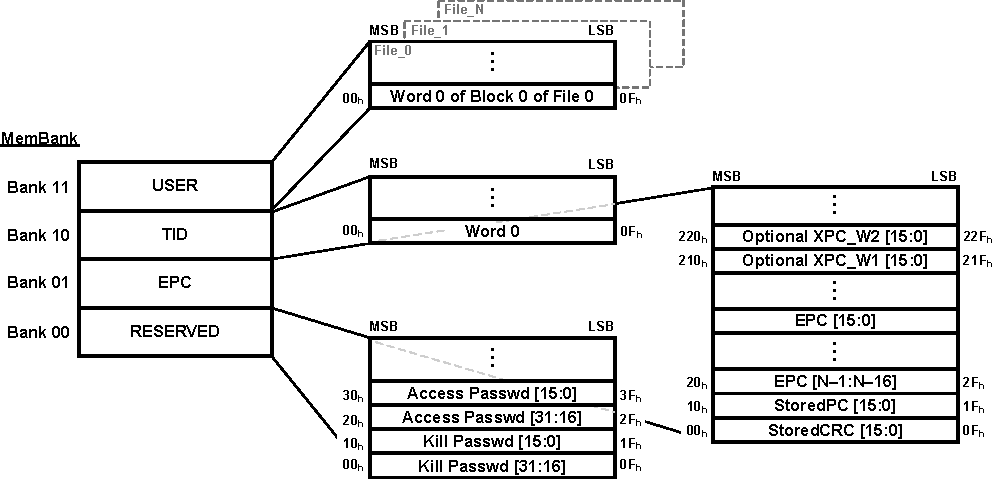
\includegraphics[width=\textwidth]{./figs/02-state-of-the-art/logicmemorymap.pdf}
    \caption[Logical memory map of EPCGlobal \ac{gen2} \ac{uhf} tags]{Logical memory map of EPCGlobal \ac{gen2} \ac{uhf} tags~\cite{UHFGen2Tag}} 
    \label{fig:logicalmemorymap}
\end{figure}

\subsubsection{Reserved Memory}

Reserved Memory (Bank $00$) holds the Access and Kill passwords, if implemented by the manufacturer of the Tag. 
The \emph{Kill password} is a 32-bit value used in the \emph{Kill Command} to render a tag non-responsive thereafter. The \emph{Kill Command} only executes if the password has been set to a value different from the default all-zero password.
The \emph{Access password} is a 32-bit value which allows a tag to transit in to the Secure state. In the Secure state all Access commands can be executed, including writing to locked blocks. The default password is all zeros and must be changed if access protection is desirable~\cite{RFIDEPCGen2,UHFGen2Tag}.

\subsubsection{\ac{epc} Memory}

The \ac{epc} Memory (Bank $01$) contains a 16-bit \ac{crc} for error correction, a 16-bit \ac{pc} and an \ac{epc}.

\ac{epc} binary encoding will be further discussed in section~\ref{sec:binencoding}, it is the \ac{id} in which the \emph{EPCGlobal Framework} revolves around to identify every item in the world. The \ac{epc} is by design extensible, being that, depending on the application requirements, it can be between $96$ bits and the maximum \ac{epc} size supported by the tag (some tags can have \ac{epc} memory up to $496$ bits). Important to refer, tag cost rises with the amount of \ac{epc} bits. Companies planning on implementing \ac{epc} must devise a serialization plan where a estimate of serial numbers and unique products is done. This will influence the requirements in \ac{epc} memory and consequently tag price.
The encoding of \ac{epc} is not defined in the \ac{gen2} air protocol standard, but in the \emph{\ac{epc} Tag Data Standard} which will be further discussed with detail on section~\ref{sec:epc}.

The standard also defines \ac{xpc} words, \acs{xpc}\_W1 and \acs{xpc}\_W2 respectively. These words are optional and usually not implemented by tag manufacturers. In fact, the tags used in this dissertation - with \textit{Impinj's Monza} chips - are widely used in all kinds of tag applications around the globe, and don't implement \ac{xpc} words. These words contain bit indicators for settings like hazardous materials and intractability to say a few.

The \ac{pc} word contains metadata used to interpret the \ac{epc}. A more detailed representation of the \ac{pc} can be seen in table~\ref{tab:pcbits}.
From $10_h-14_h$, 4 bits with the length of the \ac{epc}/\ac{id} in words, at $15_h$ a toggle bit called \ac{umi} which indicates if \emph{User Bank $11$} has any data in it, and at $16_h$ a toggle bit to indicate if the tag has extended \ac{pc}.
To distinguish a GS1 from an ISO standard \ac{id}, the most reasonable way is to look at bit $17_h$, which contains a toggle bit to indicate whether the \ac{id} is GS1 or non-GS1 family.
From bit $18_h$ to $1F_h$ is reserved for future use under the \emph{EPCGlobal} specification. Under some circumstances GS1 EPCglobal may permit other standard body or organization to use one or more of these RFU values for standardization purposes. Also to note, on ISO 18000-6, these bits are used for \ac{id}'s supplementary meta data called Application Family Identifier.

\begin{table}
    \centering
    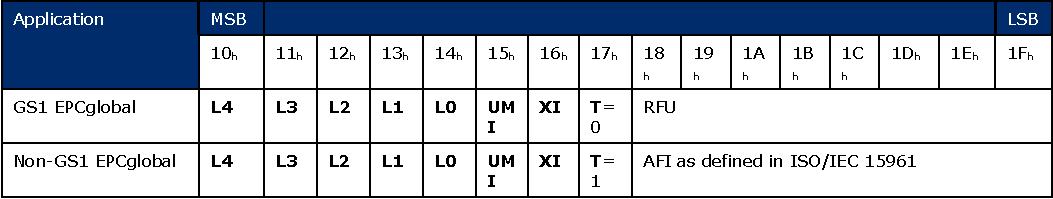
\includegraphics[width=\textwidth]{./figs/02-state-of-the-art/table_pcbits.pdf}
    \caption[\ac{pc} assignments from \ac{epc} \ac{uhf} \ac{gen2} Air Interface Protocol]{\ac{pc} assignments from \ac{epc} \ac{uhf} \ac{gen2} Air Interface Protocol~\cite{UHFGen2Tag}} 
    \label{tab:pcbits}
\end{table}

\subsubsection{TID Memory}

\ac{tid} Memory (Bank $10$) holds chip manufactured information and tag capability indicators. This memory bank is permalocked at the time of manufacture, in that it can not be changed.

The \ac{tid} Memory bank contains two fields - \ac{mdid} and \ac{tmn} - which are commonly associated together and called \ac{tid}.
\ac{mdid} encodes the tag chip manufacturer \ac{id} which is assigned by GS1 as a unique identifier.
The \ac{tmn} is attributed by the manufacturer of the chip and describes the chip identification number.

The \ac{tds}, where the encoding of \ac{tid} is specified, is often referred as \emph{Short} Tag Identification, because the \ac{tid} can be extended.

The \ac{tid} extension is called \ac{xtid} and is intended to provide more information about the capabilities of tags. It adds support for serialization and information about key features implemented by the tag~\cite{EPCTagData}.
Serialization is unique number generated by the tag manufacturer and can be used to uniquely identify one tag from another.
This identifies the tag itself, rather than item it is applied to.
\ac{xtid} implementations are common among tag manufactures. So common in fact, people started referring to the \ac{mdid}, \ac{tmn} and serialization  combination as \emph{\ac{tid} number}.
The \ac{xtid} is specially useful in cases where the \ac{epc} is not serialized or invalid.
An example of a \ac{tid} memory bank with \ac{xtid} can be seen in figure~\ref{fig:tid}.

\begin{figure}
    \centering
    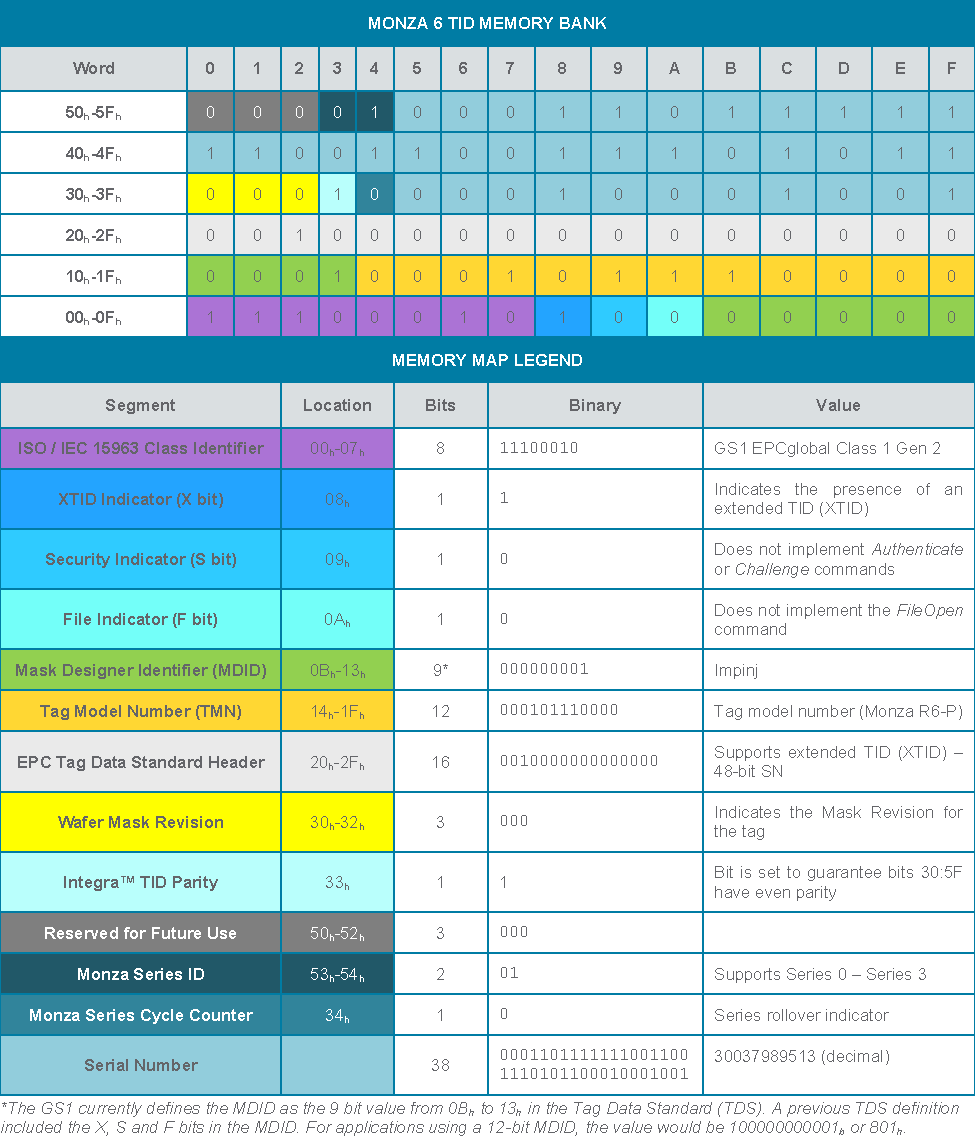
\includegraphics[width=\textwidth]{./figs/02-state-of-the-art/tid.pdf}
    \caption[\ac{tid} Memory Bank of Monza R6-P Series used in this dissertation]{\ac{tid} Memory Bank of Monza R6-P Series used in this dissertation~\cite{TIDMemoryMaps}} 
    \label{fig:tid}
\end{figure}

\subsubsection{User Memory}

The User Memory Bank provides a variable size memory to store additional data related to the tagged object.
It is frequently used to save information like temperature, maintenance logs, expiration dates and other type of data.
The bank implementation is optional and must be indicated in the \ac{umi} bit in the \ac{pc} Word.

To ensure compatibility with other protocols, the first eight bits of the bank shall contain a \ac{dsfid} as specified in ISO15962~\cite{isoISOIEC15962}.
This dissertation does not make use of the User Memory Bank, whereby it will not be covered.
For further reference, GS1 presents a solution for encoding \ac{scm} data in the User Memory Bank in the \ac{tds}~\cite{EPCTagData}.

The access to the bank is made in blocks, through the \ac{gen2} Air Protocol. The arrangement of the data in the Bank is important, as it can impact reading speeds.
GS1 provides a user memory encoder, a software which converts application data, into suitable encoded data ready to be stored in the User Memory Bank of \ac{gen2} \ac{rfid} tags~\cite{marco.santos.diamondFAQ2020}.

\section{\acf{epc}} \label{sec:epc}

% Check page 24 of the GS1 EPCglobal architecture Framework pdf

\ac{epc} is a universal identifier used to identify every physical object anywhere in the world.
Differently from common \ac{uuid} identifiers, \ac{epc} has a set of collective terms for the identification code, standardized by GS1~\cite{GS1GeneralSpecifications}. These terms convey context about the physical object in the encoding of the \ac{epc} itself.

\subsection{\ac{epc} in EPCGlobal Architecture Framework}

\acp{epc} are presented throughout the EPCGlobal Framework in various levels of abstraction. From low-level binary encoded, in \ac{gen2} \ac{rfid} tags, to text based \acp{uri} in business level applications.
The Framework presents seven representations~\footnote{binary, tag-encoding \ac{uri}, pure-identity \ac{uri}, legacy, legacy AI, element string and \ac{ons} hostname} for a single \ac{epc}. In general, only three are primarily used: \emph{Pure Identity}, \emph{Tag \ac{uri}} and \emph{Binary Encoding}.
Referring back to figure~\ref{fig:archstructure}, we observe that the three representations are used in different contexts throughout the framework.

The \emph{Pure Identity \ac{epc} \ac{uri}} format is, as the name suggests, represented in \acf{uri} format.
GS1 uses the \ac{urn} scheme with the \texttt{epc} \ac{nid} registered for the EPCglobal's \ac{epc} and related standards~\cite{meallingUniformResourceName}.
It is the most platform agnostic representation of an \ac{epc}, offering human readability and compatibility between heterogeneous systems. 

For components like middlewares, requiring more information about the \ac{epc} memory bank of \ac{gen2} \ac{rfid} tags, the \ac{tds} provides a \emph{Tag \ac{uri}} scheme.
This representation maintains the \ac{uri} representation, changing the \ac{nss} from \texttt{id} to \texttt{tag}, and adding \textit{control information} used to guide the process of data capture of \ac{rfid} tags.
This scheme preserves information regarding the \ac{epc} Memory Bank in the \ac{urn} namespaces that are usually disregarded in business applications but necessary in middleware operations.
In other words, the \emph{\ac{epc} Tag \ac{uri}} is a text equivalent of the entire \ac{epc} memory bank contents.
Examples of booth \ac{uri} representations can be seen in figure~\ref{fig:epcurirepresentation}. 

\begin{figure}[!ht]
    \centering
    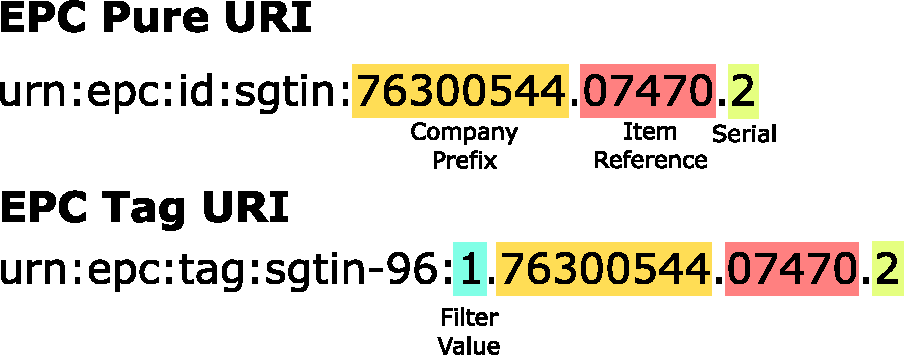
\includegraphics[width=0.8\textwidth]{./figs/02-state-of-the-art/SGTIN_First2encodings.pdf}
    \caption[\emph{Pure Identity} and \emph{Tag \acp{uri}} \ac{epc} representation]{\emph{Pure Identity} and \emph{Tag \acp{uri}} \ac{epc} representation adapted from~\cite{SGTININFO}} 
    \label{fig:epcurirepresentation}
\end{figure}

The Binary Encoding of \ac{epc} contains a compressed encoding of the EPC and additional \textit{control information} in a compact binary form, like showed on figure~\ref{fig:epcbinencoding}.
A deep analysis of the binary \ac{epc} encoding will be presented in section~\ref{sec:binencoding}.

\begin{figure}[!ht]
    \centering
    \vspace*{0.5cm}
    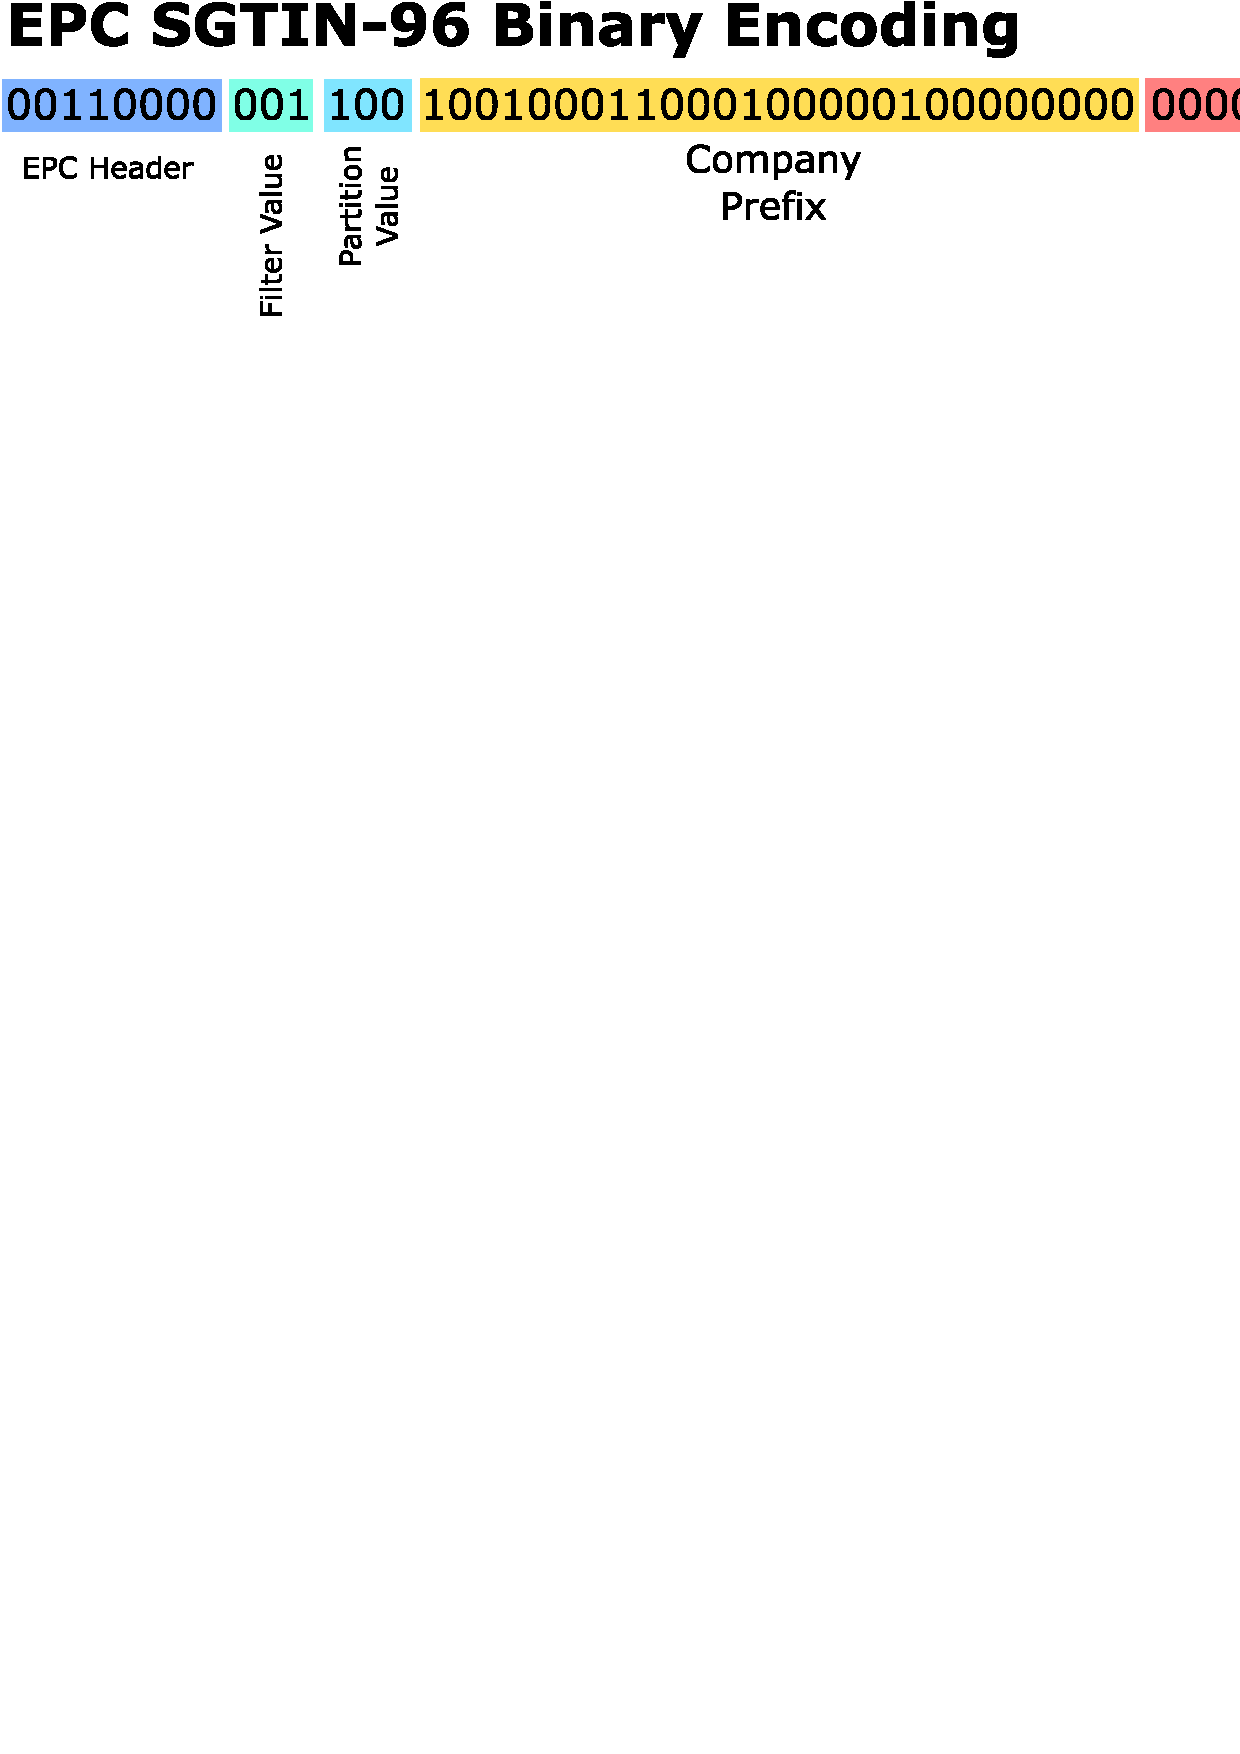
\includegraphics[width=\textwidth]{./figs/02-state-of-the-art/SGTIN_binaryconv2.pdf}
    \caption[\ac{epc} in binary encoding representation]{\ac{epc} in binary encoding representation adapted from~\cite{SGTININFO}} 
    \label{fig:epcbinencoding}
\end{figure}

\subsection{Relationship between \acsp{epc} and GS1 keys}

Before going into the encoding of \ac{epc} in \ac{gen2} \ac{rfid} tags, lets understand the underlying concepts of \ac{epc} and its schemes.

Previously, I mentioned that the \ac{epc} was designed to identify every physical object in the world.
The \emph{EPCGlobal Framework} uses this concept to its very extent.
A physical object in a \ac{scm} can be a broad term that does not provide much information regarding the object itself.
To contextualize the objects, the architecture defines GS1 keys and corresponding \ac{epc} schemes.
Each GS1 key denotes a class or grouping of physical objects. These classes encompass trade items, locations, assets, logistic units, transport groupings to say a few.
GS1 keys add valuable information to \ac{scm} operations by allowing intervening entities in the supply chain and logistics, to retrieve class context information regarding the tagged objects.

For each GS1 key there is a corresponding \ac{epc} scheme, including encoding specifications for both \ac{epc} representation: \ac{uri} and a binary encoding, for use in \ac{rfid} tags.
Each \ac{epc} scheme and corresponding GS1 key can be seen in Appendix~\ref{anx:epccodingschemes}.

\subsection{\acs{sgtin}} \label{sec:sgtin}

In the scope of this dissertation, the \ac{sgtin} scheme is the most important encoding scheme to look at.
The \ac{sgtin} encodes a \ac{gtin} plus a unique product or serial number.

\begin{figure}[!ht]
    \centering
    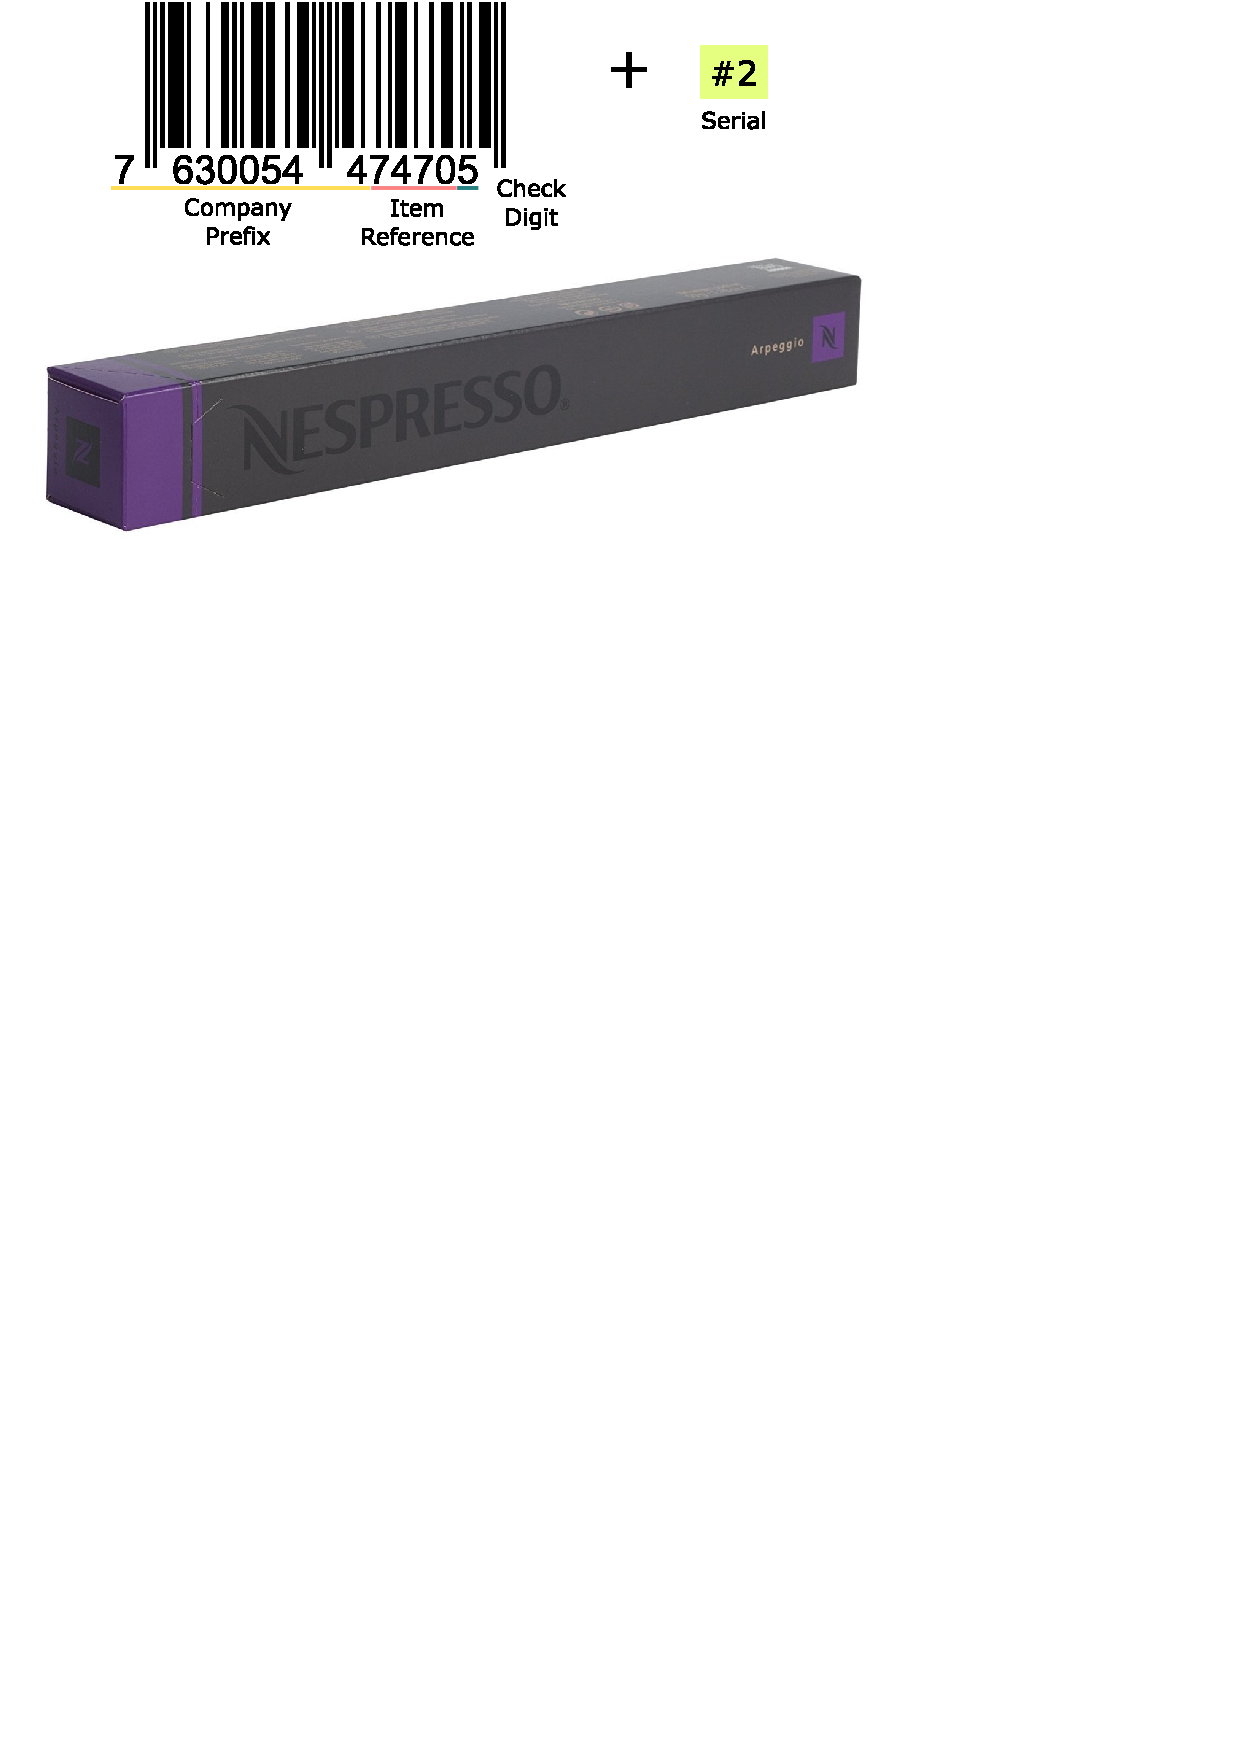
\includegraphics[width=0.8\textwidth]{./figs/02-state-of-the-art/SGTIN_UPC_Compare.pdf}
    \caption[Relation and interoperability between \ac{sgtin} and barcode's \ac{gtin}]{Relation and interoperability between \ac{sgtin} and barcode's \ac{gtin}} 
    \label{fig:barcodesgtin}
\end{figure}

The \ac{gtin} is used by companies to identify trade items~\cite{GS1GTINExecutive, GS1GTINManagement}. 
GS1 defines trade items as products or services that are priced, ordered or invoiced at any point in the supply chain.
\ac{gtin} can be used to identify types of products at any packaging level (e.g., consumer unit, inner pack, case, pallet~\footnote{even if a \ac{gtin} can be used to identify pallets, the use of \ac{sscc} is preferable~\cite{GS1KeysImplementation}}).

There are four \ac{gtin} formats: \ac{gtin}-$8$, \ac{gtin}-$12$, \ac{gtin}-$13$ and \ac{gtin}-$14$. In \ac{rfid} applications and \ac{it} applications, it is used the generalized 14-digit \ac{gtin} format. \ac{gen2} \ac{rfid} \ac{sgtin} encoding scheme is specified for \ac{gtin}-$14$.
Other \ac{gtin} formats are mainly used in barcodes in point-of-sale applications: in the \ac{us} is commonly used a \ac{gtin}-$12$ with UPC barcodes for single products and \ac{gtin}-$14$ with ITF-14 barcodes for product grouping. In contrast, in the rest of the world is commonly used \ac{gtin}-$8$ with \ac{ean}-8 barcodes for single products and \ac{gtin}-$13$ with \ac{ean}-13 for single products packaging configurations~\cite{BarcodeGS1General,GS1BarcodeChart}.

A \ac{gtin} is composed of three fields: \emph{Company Prefix}, \emph{Item Reference} and check digit. All these fields are encoded in the same manner in the different N-digit \ac{gtin} formats. A \ac{gtin}-$13$ can be converted in a \ac{gtin}-$14$ by adding a leading zero, and other \acp{gtin} formats follow the same logic.

GS1 \emph{Company Prefix} is an identifier licensed by GS1 to identify a company globally. 
Nowadays, the registration of such is essential to companies wishing to sell products in big retail stores and digital marketplaces like Ebay and Amazon~\cite{ListingRequirementsProduct}).
A \emph{Company Prefix} does not uniquely identify a manufacturer. Companies can register and own more than one \emph{Company Prefix}~\cite{GS1EPCglobalArchitecture}, and in certain circumstances \emph{Company Prefixes} can change.
When licensing a \emph{Company Prefix}, there is an assessment and plan of unique product items a company shall produce. 
Depending on that, GS1 attributes a prefix with a length adjusted to company requirements. 
Companies requiring high quantities of unique item are given a shorter Company Prefix, accommodating more digits for item identification.
Also worth mentioning, the attribution of \emph{Company Prefixes} is made by one of the GS1 branches. Each branch has a prefix which uses to assign \emph{Company Prefixes} (e.g.\ GS1 Portugal has $560$, GS1 Schweiz, Suisse and Svizzera have $760$-$769$)~\cite{anonymousGS1CompanyPrefix2014}.

\emph{Item References} are assigned by the managing entity of the product.
The item reference must be concatenated with the \emph{Company Prefix} to calculate the Check Digit, forming a \ac{gtin}.
From a \ac{gtin}, an \ac{sgtin} can be commissioned~\footnote{``Commisioning'' is the technical term used when creating new \acp{epc} for objects}, allowing to uniquely identify a product within its product grouping.
Important to clarify, when a \ac{gtin} is stored in \ac{rfid} tags, as in \ac{sgtin} coding schemes, the Check Digit has no purpose, so it is dropped. The Check Digit exists for error checking in barcodes. When converting barcode \ac{gtin} to \ac{epc} \ac{sgtin} encoding scheme, the Check digit must be dropped.

\subsection{Binary Encoding} \label{sec:binencoding}

Lets now understand how \acp{epc} are stored in \ac{gen2} \ac{rfid} tags.
We will focus on \ac{sgtin} encoding scheme, but the encoding method is analogous to other encoding schemes.

The binary encoding of an \ac{epc} consists of a fixed length header followed by a series of fields inherent to the encoding scheme like showed on \ac{sgtin}-$96$ Coding table~\ref{tab:sgtin96codingtable}.
For instance, lets take the \emph{Tag \ac{uri}}
\mintinline{python}{urn:epc:tag:sgtin-96:1.76300544.07470.2}
has example.
This \emph{Tag \ac{uri}} presents a \ac{sgtin}-$96$ encoding scheme, \emph{Filter value} of $``1"$, \emph{Company Prefix} $``76300544"$, \emph{Item Reference} $``7470"$ and serial $``2"$.

\begin{table}[]
    \centering
    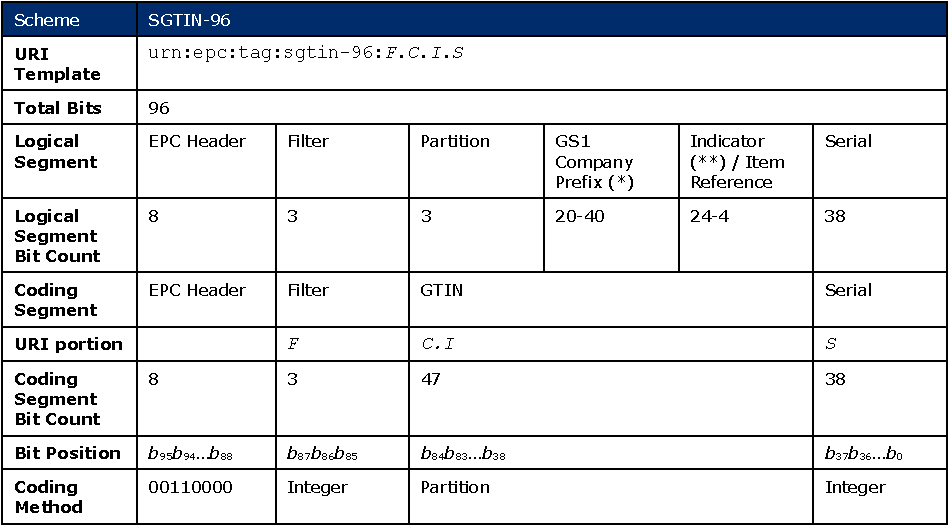
\includegraphics[width=\textwidth]{./figs/02-state-of-the-art/table_codingtable.pdf}
    \caption[Coding Table of \ac{sgtin}-$96$]{Coding Table of \ac{sgtin}-$96$~\cite{EPCTagData}} 
    \label{tab:sgtin96codingtable}
\end{table}

Following table~\ref{tab:encodingexample}, showing the \emph{Tag \ac{uri}} encoding, we first need to address the \ac{epc} header value.
A snippet of the \ac{epc} header values can be seen in table~\ref{tab:epcheaders}. We observe that an \ac{sgtin} with $96$-bit coding scheme encodes a $8$-bit header with binary value of $``00110000"$.

\begin{table}[]
    \begin{adjustwidth}{-0.09\textwidth}{0em}
    \begin{tabular}{@{}lllrl@{}}
        \toprule
        \textbf{Field}                                            & \textbf{Value (dec)} & \textbf{Value (bin)}                                                              & \textbf{\begin{tabular}[c]{@{}r@{}}Length \\ (bits)\end{tabular}} & \textbf{Notes}                                                                                                      \\ \midrule
        \ac{epc} Header                                                & 48                   & 00110000                                                                          & 8                                                                 & \ac{sgtin}-$96$ encoding                                                                                                 \\
        Filter Value                                              & 1                    & 001                                                                               & 3                                                                 & \ac{pos} item                                                                                                            \\
        Partition Value                                           & 4                    & 100                                                                               & 3                                                                 & Company Prefix has 8 digits                                                                                         \\
        \begin{tabular}[c]{@{}l@{}}Company \\ Prefix\end{tabular} & 76300544             & \begin{tabular}[c]{@{}l@{}}1001000110001000\\ 00100000000\end{tabular}            & 27                                                                &                                                                                                                     \\
        \begin{tabular}[c]{@{}l@{}}Item\\ Reference\end{tabular}  & 7470                 & 00001110100101110                                                                 & 17                                                                & \begin{tabular}[c]{@{}l@{}}Length depends on the partition\\ MSB zero fill\end{tabular}                             \\
        Serial                                                    & 2                    & \begin{tabular}[c]{@{}l@{}}0000000000000000\\ 0000000000000000000010\end{tabular} & 38                                                                & \begin{tabular}[c]{@{}l@{}}Serial is of fixed length.\\ Can be extended with \\ bigger EPC Memory Bank\end{tabular} \\ \bottomrule
        \end{tabular}
    \end{adjustwidth}
    \caption[\ac{sgtin}-$96$ binary encoding example of \texttt{urn:epc:tag:sgtin-96:1.76300544.07470.2} \emph{Tag \ac{uri}}]{\ac{sgtin}-$96$ binary encoding example of \texttt{urn:epc:tag:sgtin-96:1.76300544.07470.2} \emph{Tag \ac{uri}} retrieved from the Platform developed in this dissertation} 
    \label{tab:encodingexample}

\end{table}

\begin{table}[]
    \centering
    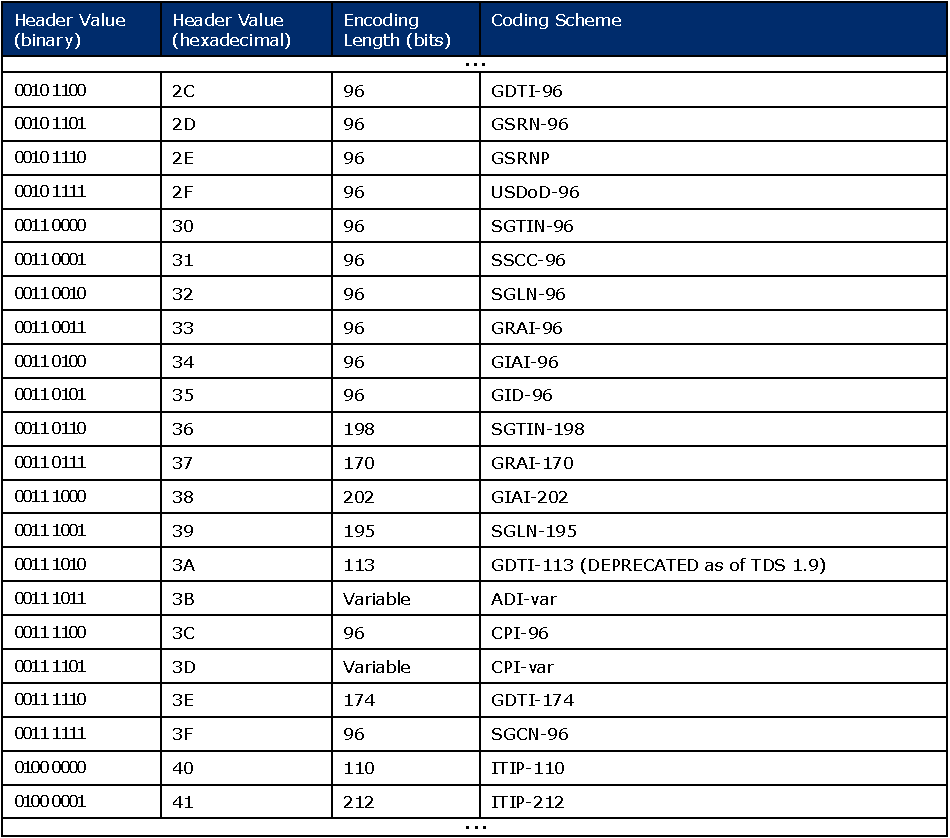
\includegraphics[width=\textwidth]{./figs/02-state-of-the-art/table_epcheaders.pdf}
    \caption[\ac{epc} headers snippet]{\ac{epc} headers snippet adapted from \ac{tds}~\cite{EPCTagData}} 
    \label{tab:epcheaders}
\end{table}

Next, we need to encode the additional \textit{information} included in the \ac{epc} Memory Bank: \emph{Filter} and \emph{Partition}. 

The \emph{Filter} encodes the packing level. An \ac{epc} \ac{sgtin} can be used to identify different levels of item packaging sharing the same \ac{gtin}. Differently from barcodes, which only encode the \ac{gtin}, an \ac{epc} with \emph{Filter} field allows a coherent \ac{gtin} across all item packages.
The \emph{Filter} value allows \ac{rfid} readers to select or deselect tags in the \emph{\ac{epc} \ac{uhf} \ac{gen2} Air Interface Protocol} corresponding to certain filter levels. This makes it easier to read desired tags in an environment where there may be other tags present (e.g.\ logistics companies only wanting to read and track Unit Loads like pallets).
Referencing table~\ref{tab:sgtinfiltervalues}, with a filter value of $``1"$, it encodes a \ac{pos} Trade Item with binary encoding of $``001"$.

The \emph{Partition} value encodes a pair of variable-length numeric fields referent to the \emph{Company Prefix} and \emph{Item Reference} memory partition. Previously we mentioned that \emph{Company Prefixes} can vary in length depending on company requirements for unique \emph{Item References}. 
In barcodes the \emph{Company Prefix} and \emph{Item Reference} are encoded together in a \ac{gtin} value. 
In \ac{gen2} tags, although there is fixed size memory shared between \emph{Company Prefix} and \emph{Item Reference}, there is also the \emph{Partition} value, which specifies the distribution of that partition between booth fields.
In the case of the \emph{Tag \ac{uri}} example, \emph{Company prefix} has $27$ bits ($8$ digits) and \emph{Item reference} has $17$ bits ($5$ digits). Referring to table~\ref{tab:partitiontable} with the pair of variable-lengths, the \emph{Partition Value} is $``4"$ encoded has $``100"$.

\begin{table}[]
    \centering
    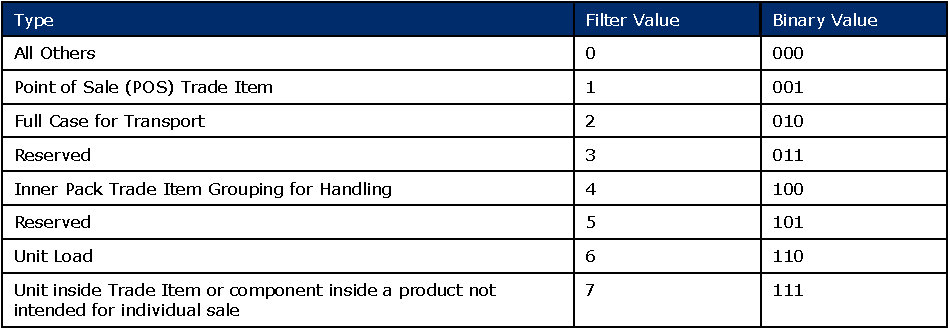
\includegraphics[width=\textwidth]{./figs/02-state-of-the-art/table_sgtin_filtervalues.pdf}
    \caption[\ac{sgtin} Filter Value Table]{\ac{sgtin} Filter Value Table~\cite{EPCTagData}} 
    \label{tab:sgtinfiltervalues}
\end{table}

\begin{table}[]
    \centering
    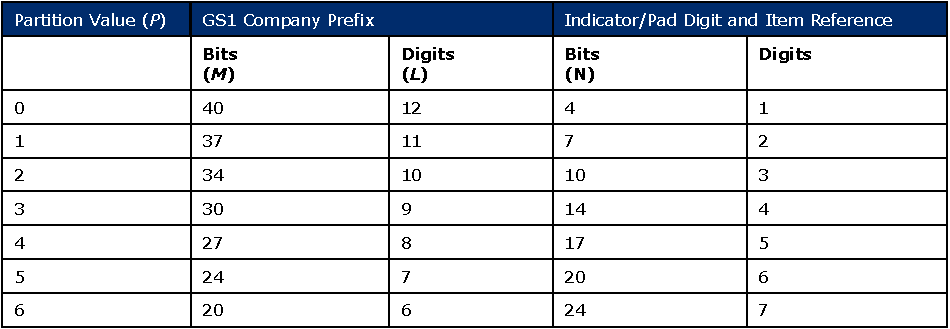
\includegraphics[width=\textwidth]{./figs/02-state-of-the-art/table_partitionvalues.pdf}
    \caption[\ac{sgtin} Partition Table]{\ac{sgtin} Partition Table~\cite{EPCTagData}} 
    \label{tab:partitiontable}
\end{table}

The \emph{Company Prefix}, \emph{Item Reference} and \emph{serial} are encoded converting from decimal to binary and add leading zeros to fill all bits in each Logical Segment.

\section{Low Level Reader Protocol (LLRP)} \label{sec:llrp}

The \acf{llrp} is specification for the network interface between \ac{rfid} Readers and Client applications~\cite{ImpinjLTKProgrammers}. \ac{llrp} is not exclusive to the \ac{gen2} Air Protocol. It was designed to support multiple \ac{rfid} air protocols, including future versions of \ac{gen2} Air Protocol.

\subsection{Design Requirements}

In some \ac{rfid} systems, there is a requirement for explicitly tune \ac{rfid} air protocols and the ability to control Readers that implement \ac{rfid} air protocol communications~\cite{LowLevelReader}. \ac{llrp} provides tuning features and commands for that purpose.

Devices intended to operate and communicate with \ac{rfid} Readers can vary from software applications, to middleware on local hardware, \acp{plc} and even cloud services. \ac{llrp} is ``simple'' enough to be implemented in all kinds of computer architectures.

\ac{llrp} was design without requiring real-time interaction between the application software and Reader, and but with time-critical tasks at heart. 
The Reader application software passes operational rules to the Reader in non-real time.
The Reader then triggers and runs those operation rules to achieve time-critical requirements. 
The triggers can come from the applications directly, from timers, \ac{gpi} hardware, or any other trigger defined by the Reader. 
This declarative operation method allows Readers to achieve peak performance without constraints caused by network or host latency.

\subsection{Connection Details}

\ac{llrp} is a binary protocol which runs over the \acs{tcp}/\acs{ip} internet transport protocols.
It is an asymmetric protocol where the \ac{llrp} client send commands to the Reader.

The protocol supports both reader and client initiated connections. By default, \ac{llrp} clients connect to \acs{tcp} port $5084$. In reader initiated connections, the Reader will actively try to establish a connection with the host application.
\ac{llrp} does not specify the behavior delivering data when a connection if broken. The reader used in this dissertation and others I've seen will continue to collect tag data and optionally deliver upon resumption of the connection.

Readers only allow one \ac{llrp} connection at any time. The \ac{tcp} connection between reader and client stays open until the client closes it or connection drops.

\subsection{Operation}

The primary function of the \ac{llrp} interface is to allow a client to finely tune the \ac{gen2} Tag Air Standard parameters, and command the reader to perform an inventory and otherwise access tags for read, write, lock, and kill.

To meet these requirements, \ac{llrp} defines \acp{spec}, containing descriptions of ``what, how and when'' the Reader should perform certain operations.
\acp{spec} are run when triggered. The trigger range from boundary trigger information defined in the \ac{spec} itself, \acp{gpi}, or by immediate triggers from applications for a more imperative behavior.
\acp{spec} are sent inside of messages, which are the unit of communication between client and Reader.
\ac{llrp} contains forty basic messages which range from commands, responses, events and a \textit{CUSTOM\_MESSAGE} for vender extensions. A list and description of every message can be found in Appendix~\ref{anx:llrpmessages}.

In figure~\ref{fig:ROACCESSREPORTbin} we observe an example of binary encoding of the \textit{RO\_ACCESS\_REPORT} message.
Inside the message there is a \ac{spec}, and inside a \ac{spec}, data is sent as \emph{parameters} and \emph{fields}.
\emph{Fields} are individual data elements with a known basic format.
\emph{Parameters} are named data elements that contain other parameters and/or fields, much like structures in programming languages.
Inside the \textit{RO\_ACCESS\_REPORT} message, in figure~\ref{fig:ROACCESSREPORTbin}, it can be observed the memory allocated for a list of a parameter called \texttt{TagReportData}. \texttt{TagReportData} is then encoded following figure~\ref{fig:TagReportDatabin}, which inside encodes an \texttt{EPCData} or \texttt{EPC-96} parameter, where the binary encoded \ac{epc} is allocated.
When constructing \ac{llrp} messages, parameters can be optional, but field must be presented and within their valid range. Some tooling software provides user friendly features like inferring Reader capabilities and default values for unspecified fields.

\begin{figure}[]
    \centering
    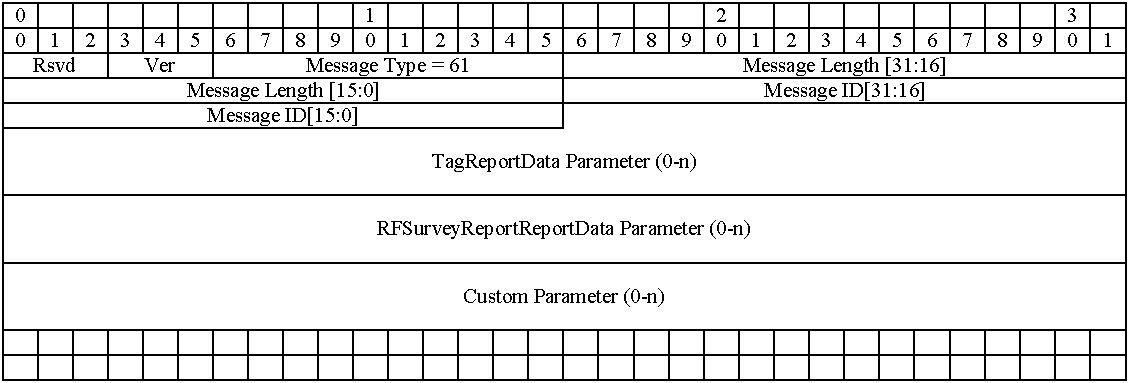
\includegraphics[width=\textwidth]{./figs/02-state-of-the-art/RO_ACCESS_REPORT_bin.pdf}
    \caption[\textit{RO\_ACCESS\_REPORT} message binary encoding]{\textit{RO\_ACCESS\_REPORT} message binary encoding~\cite{LowLevelReader}. This message is sent by the Reader and contains inventory and access operations results} 
    \label{fig:ROACCESSREPORTbin}
\end{figure}

\begin{figure}[]
    \centering
    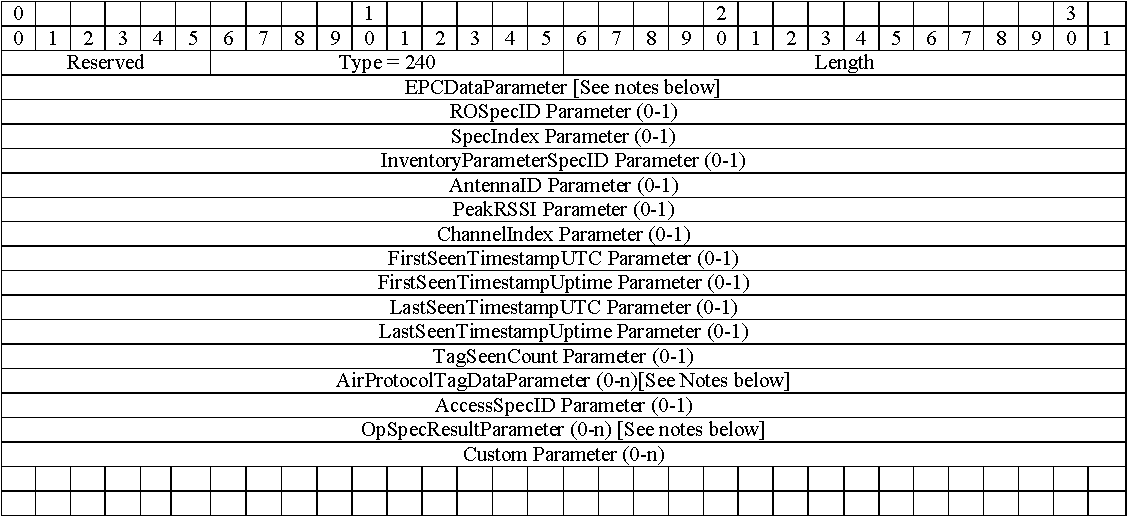
\includegraphics[width=\textwidth]{./figs/02-state-of-the-art/TagReportData_bin.pdf}
    \caption[\texttt{TagReportData} parameter binary encoding]{\texttt{TagReportData} parameter binary encoding~\cite{LowLevelReader}. \texttt{TagReportData} is generated per tag and contains a mandatory parameter \texttt{EPCData} with encoding} 
    \label{fig:TagReportDatabin}
\end{figure}

\begin{figure}[]
    \centering
    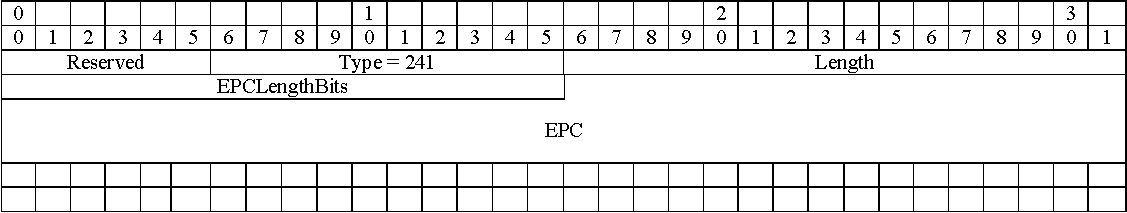
\includegraphics[width=\textwidth]{./figs/02-state-of-the-art/EPCDataParameter_bin.pdf}
    \caption[\texttt{EPCData} parameter binary encoding]{\texttt{EPCData} parameter binary encoding~\cite{LowLevelReader}. \texttt{EPCData} shall be used for encoding a non-96 bit \ac{epc}, whereas the \texttt{EPC-96} Parameter on figure~\ref{fig:EPC96bin} is be used for encoding a 96-bit \ac{epc}} 
    \label{fig:EPCDatabin}
\end{figure}

\begin{figure}[]
    \centering
    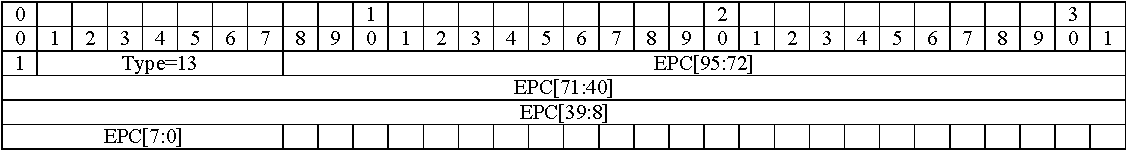
\includegraphics[width=\textwidth]{./figs/02-state-of-the-art/EPC96ParameterTVEncoding_bin.pdf}
    \caption[\texttt{EPC-96} parameter binary encoding]{\texttt{EPC-96} parameter binary encoding~\cite{LowLevelReader}}
    \label{fig:EPC96bin}
\end{figure}

\subsection{\acf{spec}} \label{sec:llrpspecs}

There are two main \acp{spec} defined in the \ac{llrp} Standard:  \textit{\acp{rospec}} and \textit{Access \acp{spec}}. Most of other \acp{spec} and parameters are enclosed under one of the two.
I will briefly discuss relevant knowledge required to understand the \acp{spec} context. Detailed information on necessary fields will be presented later in opportune moments throughout this dissertation.

\subsubsection{\acf{rospec}}

\acp{rospec} control the operation of the Reader. They describe the inventory operations the Reader has to perform.
A Reader only supports one \ac{rospec} at a time.
An example of a \ac{rospec} is presented inside the \textit{ADD\_ROSPEC} message seen in Code~\ref{code:rospec}. \ac{xml} is used in the context of many \ac{llrp} clients to provide human readability of the binary protocol, and also used in this dissertation for the same reason.
In the \textit{ADD\_ROSPEC} \ac{xml} message we observe one \ac{rospec} and constituting parameters and fields.
\acp{rospec} contain the following elements:

\begin{description}

\item[\texttt{ROSpecID}] is an \ac{id} set by the client to uniquely identify the \ac{spec} in subsequent commands.

\item[\texttt{Priority}] should be set to $``0"$~\cite{ImpinjLTKProgrammers}. By default, all \acp{rospec} should have the same priority. High priority \acp{rospec} can preempt an active lower priority one and start execution as soon as the start condition occurs.

\item[\texttt{CurrentState}] describes the current state of the \ac{rospec} - \emph{disabled}, \emph{inactive}, \emph{active}. When adding and \ac{rospec} the state must be set to \emph{disable}.

\item[\texttt{ROBoundarySpec}] is a parameter containing a description of the start and stop conditions for the \ac{spec}. 
These conditions can be, for the start trigger:
\begin{itemize}
    \item \texttt{None/Null} - \ac{rospec} will not start unless indicated by the client application through an \textit{START\_ROSPEC} message;
    \item \texttt{Immediate} - the \ac{rospec} will start immediately after enabled, and will continuously restart itself until disabled;
    \item \texttt{Periodic} - when enabled, the \ac{rospec} will be triggered periodically;
    \item \texttt{\ac{gpi}} - the enabled \ac{rospec} will start when the \ac{gpi} event enters a certain state.
\end{itemize}

For the stop triggers:
\begin{itemize}
    \item \texttt{None/Null} - the \ac{rospec} only stops when stopped by the client through the \textit{STOP\_ROSPEC};
    \item \texttt{Duration} - \ac{rospec} stops when it has been active for a specified duration;
    \item \texttt{\ac{gpi}} - \ac{rospec} will stop when the \ac{gpi} event enters a certain state.
\end{itemize}

\item[\texttt{\ac{aispec}}] contains the settings for the Reader's antennas and \ac{gen2} Air protocol options. An \ac{rospec} can have one or more \acp{aispec} which are executed when the \ac{rospec} runs.

\item[\texttt{ROReportSpec}] is optional and describes ``when'' reports should be forward to the client and ``what'' the report contains. If not defined, the Reader will use the current or default settings.
\end{description}

\begin{listing}
    \inputminted[linenos]{xml}{./code/sota/llrp_messages/ROSPEC.xml}
    \caption{Example of \textit{ADD\_ROSPEC} message in \ac{xml} representation}
    \label{code:rospec}
\end{listing}

\subsection{Application Flow}

A typical \ac{llrp} application flow can be seen in figure~\ref{fig:llrpflow}. Upon establishing a \ac{tcp} connection, a Client add and enables an \ac{rospec}, containing information about the inventory procedures. The Client can also register a \ac{aispec} for \ac{gen2} commands, like writing \acp{epc}.
The Reader, upon trigger, executes the \acp{spec}, performing \ac{epc} inventory and tag operations, which are reported back to the Client.

\begin{figure}[!ht]
    \centering
    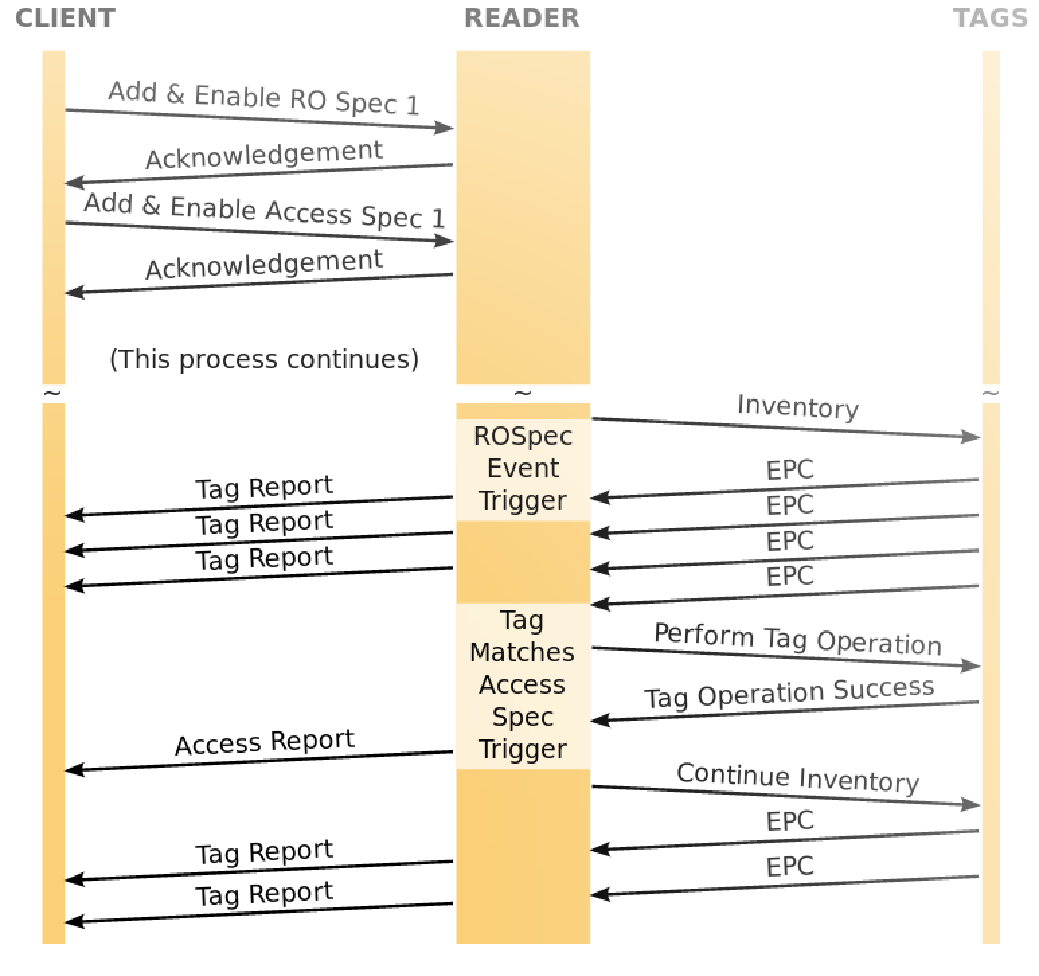
\includegraphics[width=0.9\textwidth]{./figs/02-state-of-the-art/llrpflow.pdf}
    \caption[Example of \ac{llrp} Application Flow]{Example of \ac{llrp} Application Flow~\cite{ImpinjLTKProgrammers}} 
    \label{fig:llrpflow}
\end{figure}


\subsubsection{Access \acl{spec}}

An \emph{Access \ac{spec}} handles the extended tag operations of \ac{gen2}: read, write, lock and kill.
It was design to be extensible, in order to support multiple air protocols and their respective commands.
These will not be directly used in the practical context of this dissertation, so no further description will be added.

\section{\acf{fc}}

\ac{fc} is a specification for middlewares operating between readers and client applications, to receive, filter, translate and deliver data to client applications.

\ac{gen2} \ac{rfid} readers can generate large amounts of network traffic. The amount of requests generated, containing reports with \ac{epc} raw data, can bottleneck most networks, being unsuited for internet data exchanges. 
Often, client applications are hosted in different networks and even different physical places. With the current paradigm of cloud computing, the interest in processing data on data centers only seems to be growing.
Furthermost, raw \ac{epc} data is not ``high-level'' compared to the paradigm of most business logic in client applications.
Client applications, without any middleware, have to process and contextualize huge amounts of data, overburdening services with workloads that are not in their scope of work.

\subsection{Responsibilities}

In the standard specification, EPCGlobal defines responsibilities and interfaces for \ac{fc} middlewares. Companies are free to extended these responsibilities and add features in their own implementations.

A \ac{fc} middlewares must be able to receive raw tag reads from one or multiple \ac{rfid} readers through an \ac{llrp} client interface.
These raw tags, in binary encoding, must be decoded and translated in to \ac{uri} representations, used in client applications.

Tag reads must all be processed to reduce the \ac{epc} data volume: this includes filtering, by ignoring \acp{epc} according to subscription patterns; 
aggregate \acp{epc} over time intervals, eliminating duplicate reads within that interval;
summarize and count \acp{epc} in specific object classes;
and differential analysis, by reporting which \acp{epc} have been added or removed.

\ac{fc} must be able to invoke \ac{gen2} commands on the reader, required by applications to write, lock, kill, and otherwise operate upon tags.
\ac{fc} should also map readers by \textit{logical reader names} defined in the configurations commands and/or file.

Lastly, \ac{fc} middleware must expose an \ac{ale} interface to provide means for client applications to request \ac{epc} data, reader information, control information and configure all \ac{fc} aspects described previously.

\section{\acf{ale}}

The \ac{ale} interface role is to provide independence  between the infrastructure components and the applications that use the data.
Business application have access to the lower layers of the infrastructure, like readers and middlewares, without configuring hardware or make low level logical indicators to select data.
Succinctly, the interface allows client applications to register and subscribe to their interested \ac{epc} patters and request strategies in an high-level declarative way.

\ac{ale} uses a \ac{wsdl}, an \ac{xml} based interface used to describe functionality offered by web services, to define, configure and request reports from middlwares and smart readers.
The \ac{xml} schema is defined in a \ac{xsd} file. The \ac{xsd} file expresses a set of rules to which \ac{xml} documents must conform in order to be considered valid. 
The interface also defines \ac{soap} bindings on top of the \ac{wsdl} for the callback interface for reading and writing \acp{api}.

\subsection{Specifications and Reports}

To configure and subscribe to interested \ac{epc} patterns, client applications must first register \textit{logical readers} using a \emph{\acf{lrspec}}. An example can be seen in Code~\ref{code:lrspec}. \emph{\acp{lrspec}} are basically readers registration forms.

\begin{listing}
    \inputminted[linenos, breaklines]{xml}{./code/sota/LRSpec.xml}
    \caption{Example of \emph{\acs{lrspec}} used to register a single Reader named \textit{ImpinjSpeedwayShelve1} with \ac{ip} $169.254.1.1$}
    \label{code:lrspec}
\end{listing}

To subscribe to \ac{epc} data, clients register \emph{\acp{ecspec}}. 
\acp{ecspec} take inspiration from the same ideas as in \ac{llrp}, by describing event boundaries, filtering and subscription patterns, aggregation rules and differential analysis report options in a truly high-level form.
One example can be seen in Code~\ref{code:ecspec}. The example subscribes to \ac{epc} data from the logical reader \textit{Reader\_Shelve1}. The middleware should send back to the client two types of reports every $5$ seconds: one reporting all \ac{epc} tag-\acp{uri} added to the reading zone of the reader; and other reporting all \ac{epc} tag-\acp{uri} removed from the reading zone and a count of total removed tags.
A complex \emph{\ac{ecspec}} with subscription patterns will be presented in next chapters, in the practical implementation sections of this dissertation.

\begin{listing}
    \inputminted[linenos, breaklines]{xml}{./code/sota/ECSpec.xml}
    \caption[\emph{\ac{ecspec}} example]{\emph{\ac{ecspec}} example used in early stages of the practical work of this dissertation}
    \label{code:ecspec}
\end{listing}

Subsequently, client have to indicate where the \emph{\acp{ecspec}} reports should be delivered, by indicating a \texttt{NotificationURI}.
These reports are named \emph{\acp{ecreport}} and an example can be seen in Code~\ref{code:ecreport}.

\begin{listing}
    \inputminted[linenos, breaklines]{xml}{./code/sota/EC_REPORT_deletions.xml}
    \caption[Example of \emph{\ac{ecreport}}]{Example of \emph{\ac{ecreport}} generated by the \ac{ecspec}'s \textit{detetions} Report \ac{spec} in Code~\ref{code:ecspec}, where a three tags were removed from the reading zone}
    \label{code:ecreport}
\end{listing}

\section{Capture Application}

In the \emph{EPCGlobal Framework}, the Capture Application role serves to contextualize \ac{epc} data from \emph{\acp{ecreport}} into \ac{epcis} data, and send it to an \ac{epcis} repository to be stored.
Capture Applications requirements are not further specified by the \emph{EPCGlobal Framework}.

From what I have encountered, generic capture applications implement dynamic run-time rule engines, to specify business logic in an high-level context (e.g.\ Java Drools).
Many integrate interfaces for other device-generated data such as bar codes, matrix data (e.g.\ QR Code), human input and data gathered from other software systems.
Business logic in capture applications can be complex: retail capture applications can implement anti-thief mechanism, predict out-of-stock situations, infer clients shopping experience and gather data for machine learning services (e.g.\ to infer client interests)~\cite{RFIDRetailKey}.

\section{\acf{epcis}}

\ac{epcis} enables enterprises to create and share \ac{epc} related data with trading partners.
The standard was conceived as part of a broader effort to enhance collaboration between trading partners, to create visibility of physical and digital objects within relevant business contexts~\cite{EPCISGuidelines}.

\subsection{Data Model and \acf{cbv}}

To ensure conformity in data shared across systems, the \ac{epcis} standard defines a data model. This allows disparate application to operate under coherent data structures capable of being providing visibility in relevant business operations.

\ac{epcis} structures the real-world business information as a sequence of individual business processes.
Business processes can vary. From packaging product, packing into a shipping container, shipping, receiving, and so forth.
Each completion of one of these business process is modeled by an \ac{epcis} Event.

An \ac{epcis} Event is the basic unit of data in the \ac{epcis} data model.
It provides a detailed picture of a business processes by organizing its contents into four dimensions: \emph{What}, \emph{When}, \emph{Where} and \emph{Why}.

The \emph{What} dimension identifies the physical and digital objects involved in the event. It uses the \ac{epc} \ac{tds} schemes, seen previously, to do so.  On section~\ref{sec:epc}, we talked about \ac{epc} and how it encodes information about the physical object it refers to. We focused on \ac{sgtin} for item level identification, but different GS1 Keys exit to identify a multitude of \ac{scm} assets: like pallets, batches and lots, returnable assets, to say a few (see Appendix~\ref{anx:epccodingschemes}).

\emph{When} dimension records when the event took place. It contains three elements: \texttt{Event Time} contains the date and time at with the event took place; \texttt{Event Time Zone Offset} indicates the time zone at the place and time of the event; and \texttt{Record Time} which saves the date and time when the \ac{epcis} event was recorded into an \ac{epcis} repository.

\emph{Where} dimension, as it implies, captures where the event physically took place and/or where are the objects following the event. The dimension allows for two location types: \texttt{Read Point} and \texttt{Business Location}.
The \texttt{Read Point} is the location where the event took place. The \texttt{Business Location} is the location where the objects reside after the event.

Locations are preferably identified by a \ac{gln}. A \ac{gln} is a GS1 Identification Key used to identify physical location like factories, businesses and facilities~\cite{GS1KeysImplementation}. \acp{gln} are often accompanied by an extension used to identify internal physical locations within a location identified by the \ac{gln}. An example of a \ac{gln} can be seen in figure~\ref{fig:gln}. 

\begin{figure}[]
    \centering
    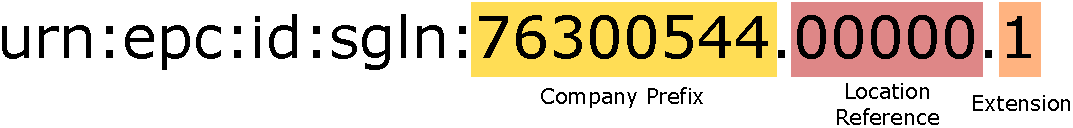
\includegraphics[width=0.8\textwidth]{./figs/02-state-of-the-art/sglnexample.pdf}
    \caption[Example of \ac{gln} with extension (SGLN) in \ac{uri} format]{Example of \ac{gln} with extension (SGLN) in \ac{uri} format. In the practical context of this dissertation, identifies the improvised shelve reading point in a Nespresso boutique store} 
    \label{fig:gln}
\end{figure}

The \emph{Why} dimension describes the context of the business process in which the event took place.
This dimension includes a multitude of parameters, which are included in the \ac{epcis} Event as a combination of such~\footnote{Some of parameters change between \ac{epcis} and \ac{cbv} versions due to reformulations in both standards}:

\begin{itemize}
    \item \textbf{Business Step} identifies what was taking place from a business context (e.g.\ \texttt{packing}, \texttt{shipping}, \texttt{inspecting}, \texttt{retail\_selling}).
    \item \textbf{}{Disposition} identifies the business condition ensuing the event of the object (e.g.\ \texttt{recalled}, \texttt{retail\_sold}, \texttt{in\_transit}, \texttt{stolen}).
    \item \textbf{Business Transaction List} identifies business transactions relevant to an event. It is described by a pair of identifiers: \texttt{Business transaction type} which identifies the type of transaction; and \texttt{Business transaction ID}, and \ac{id} that identifies a specific transaction.
    \item \textbf{Source} and \textbf{Destination} are used to provide additional business context when the event is part of a business transfer of ownership, responsibility or custody.
\end{itemize}

The possible values of these parameters are standardized under the \ac{cbv} Standard, which operates in association with the \ac{epcis} to provide common and standardized business vocabulary~\cite{CoreBusinessVocabulary}. The \ac{cbv}, much like most of \emph{EPCGlobal Framework}, uses a \ac{uri} syntax has parameter values.
An example of a populated \ac{epcis} Event can be seen in table~\ref{tab:epciseventinfo}.

\begin{table}
    \centering
    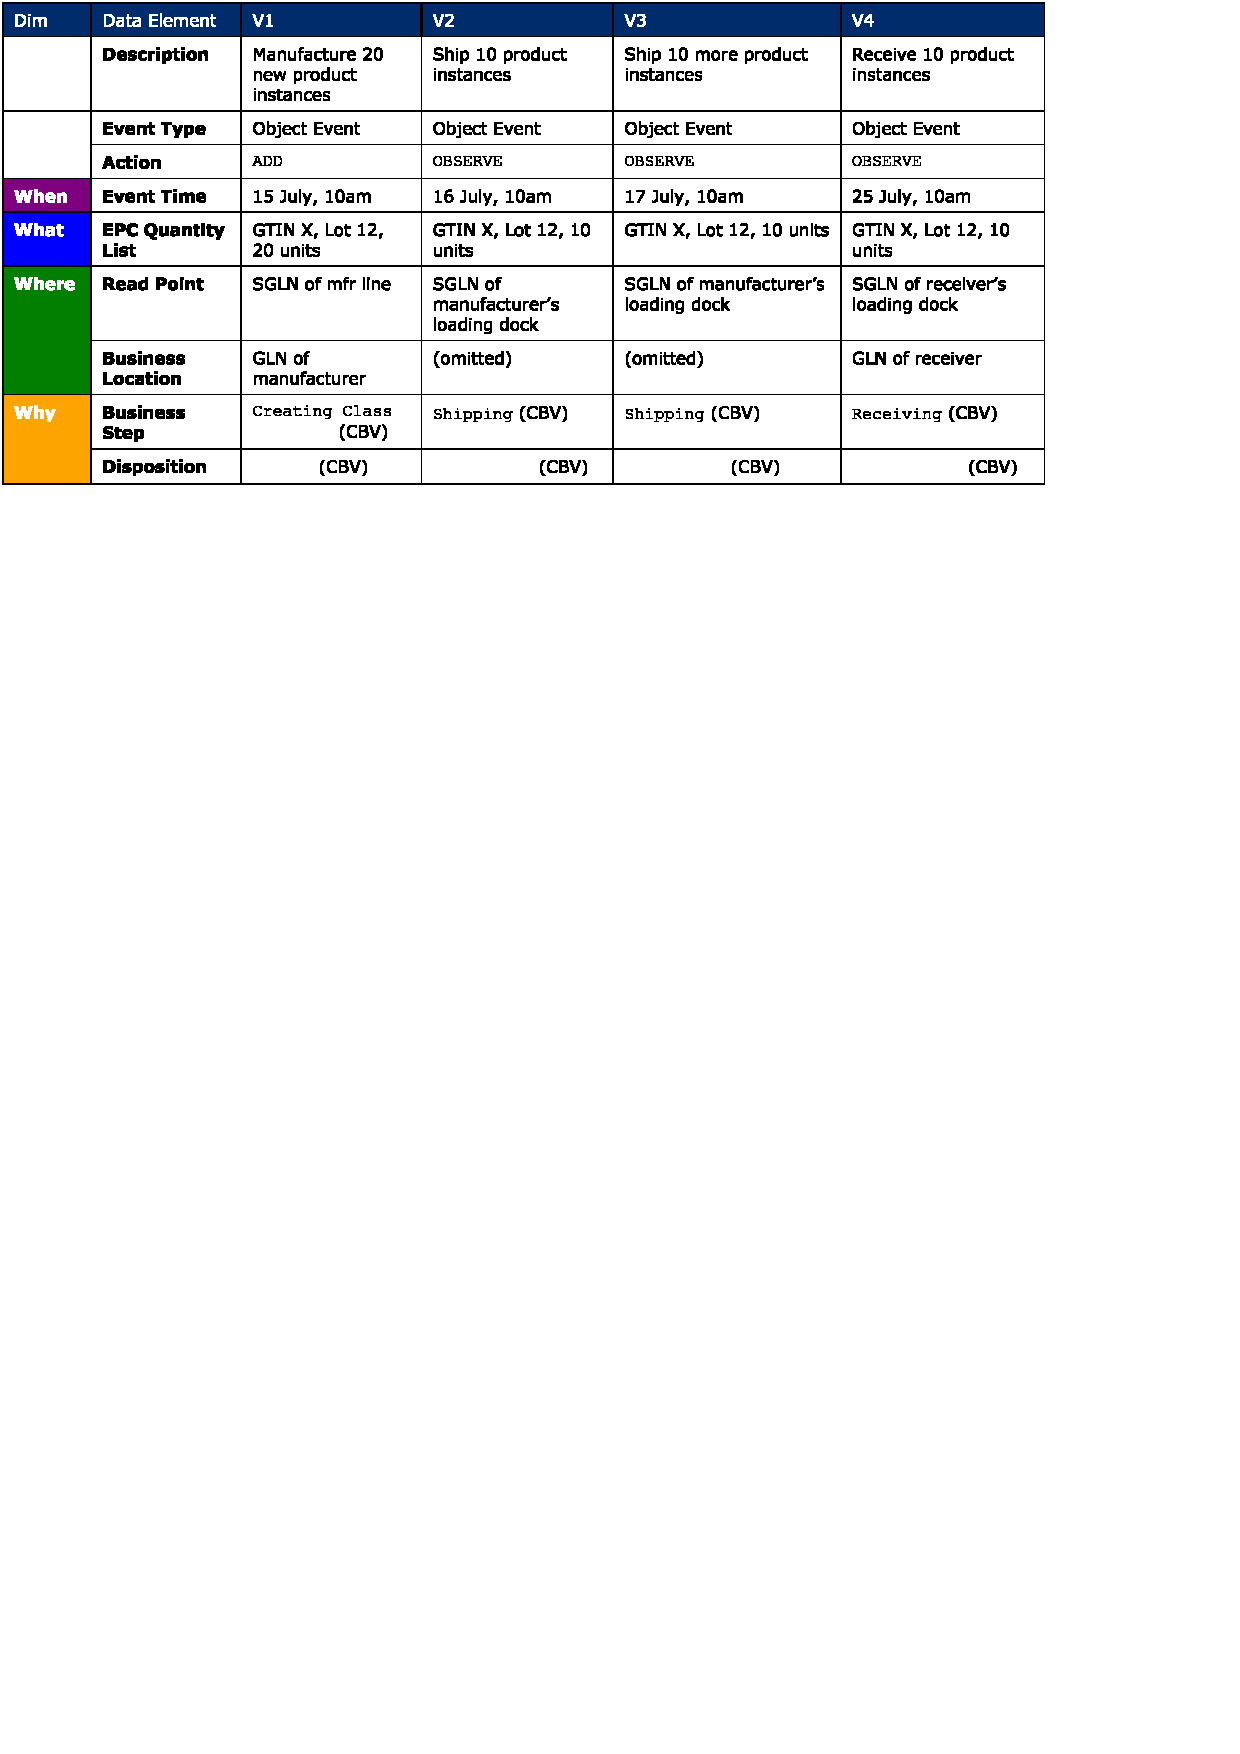
\includegraphics[width=\textwidth]{./figs/02-state-of-the-art/epcis_data_visibility.pdf}
    \caption[\ac{epcis} Event Information Content example]{\ac{epcis} Event Information Content example from the business process of shipping a pallet~\cite{EPCISGuidelines}}
    \label{tab:epciseventinfo}
\end{table}

\subsection{Event types}

To allow for more flexibility and variations in the structure of the \emph{What} dimension, \ac{epcis} defines a few variations of the basic \ac{epcis} Event:

\begin{itemize}
    \item \textbf{ObjectEvent} is the most simple commonly used. It represents an event that happened to one of more objects (e.g.\ shipping a pallet using a \ac{sscc}).
    \item \textbf{AggregationEvent} represents an event that happened to physically aggregated objects (e.g.\ aggregating cases in to a pallet, or removing cases from a pallet).
    \item \textbf{TrasformationEvent} represents an event in which the input objects are fully or partially consumed to produce output objects (e.g.\ processing raw materials in a product to be commercialized).
    \item \textbf{TransactionEvent} represents an event in which one or more objects become associated or disassociated with one or more business transactions (e.g.\ linking a pallet and cases to a commercial invoice)
\end{itemize}

\subsection{Capture and Query Interfaces}

To complement the data model, \ac{epcis} also standardizes two interfaces: a \emph{Capture interface} that allows client to send \ac{epcis} Events, to be saved, typically in a persistent repository of \ac{epcis} data, called \ac{epcis} repository; and a \emph{Query interface} from which \ac{epcis} data may be requested by applications and trading partners.

The data shared between clients and these interfaces is expressed in \ac{xml}. \ac{epcis} provides \ac{xml} bindings for the data models described previously.
The \emph{Capture interface} can be used with either message queue or \ac{http}. In Code~\ref{code:epcisreport} can be seen an \ac{xml} \ac{epcis} Event example sent to a capture application. 

\begin{listing}
    \inputminted[linenos, breaklines]{xml}{./code/sota/EPCIS_query_response.xml}
    \caption[Example of an \ac{epcis} Report sent to a \ac{epcis} capture interface]{Example of an \ac{epcis} Report sent to a \ac{epcis} capture interface. \ac{epcis} Reports can be extended with User/Vendor Extensions. In this example we see a \texttt{TemperatureC} and \texttt{RelativeHumidity} vendor extensions}
    \label{code:epcisreport}
\end{listing}

\ac{epcis} \emph{Query interface} is defined as a web service and can be interacted with by the \ac{soap} transport mechanism using the following available operations: 

\begin{itemize}
    \item \texttt{poll}: queries for \ac{epcis} events matching specific criteria.
    \item \texttt{subscribe}: allows client to register a subscription for events matching specific criteria, which are delivered asynchronously to the client. 
    \item \texttt{unsubscribe}: removes a registered subscription.
    \item \texttt{getQueryNames}: returns a list with the supported types of queries supported by the service.
    \item \texttt{getSubscriptionIDs}: returns a list of active subscriptions.
    \item \texttt{getStandardVersion}: return the \ac{epcis} version supported by the service.
    \item \texttt{getVendorVersion}: returns a vendor string identifying any non-standard extensions supported by the service (e.g.\ \texttt{TemperatureC} and \texttt{RelativeHumidity} vendor extension in Code~\ref{code:epcisreport})
\end{itemize}

A simple \texttt{poll} operation can be seen in Code~\ref{code:epcisquery}. Inside the \ac{soap} envelope we can observe a \texttt{poll} operation requesting every \texttt{ObjectEvent} collected by the reading point \texttt{urn:epc:id:sgln:76300544.00000.1}. 

\begin{listing}
    \inputminted[linenos, breaklines]{xml}{./code/sota/EPCIS_query.xml}
    \caption{Example of \ac{epcis} Query requesting all \texttt{ObjectEvents} from the Business Location \texttt{urn:epc:id:sgln:76300544.00000.1}}
    \label{code:epcisquery}
\end{listing}

In the next chapter I will present the state of the art of \ac{rfid} smart shelves, purpose hardware and research.

\cleardoublepage
%

\chapter{Introdução}
\label{chapter:introduction}

\begin{introduction}
A sort description of the chapter.

A memorable quote can also be used.
\end{introduction}



\section{Acrónimos}

Primeira e seguintes referências: \ac{h2o}, \ac{h2o}

Plural, acrónimo expandido e curto: \acp{h2o}, \acs{h2o}, \acl{h2o}

Com citação \footnote{Necessária entrada na bibliografia}: \ac{adsl}, \ac{adsl}


\section{Fontes}

\begin{itemize}
\item{\tiny Tiny}
\item{\scriptsize Scriptsize}
\item{\footnotesize Footnotes}
\item{\small Small}
\item{\normalsize Normal}
\item{\large large}
\item{\Large Large}
\item{\LARGE LARGE}
\item{\huge huge}
\item{\Huge Huge}
\end{itemize}

\section{Unidades}

Utilizando o pacote \verb|siunitx| é possível utilizar unidades do Sistema Internacional. Exemplo: a aceleração da gravidade é de \SI{9.8}{\metre\per\second\squared} e um ficheiro ocupa \SI{1}{\mebi\byte}. 

\section{Code Blocks}
\lipsum[5]

\begin{listing}
\begin{minted}{c}

#include <stdio.h>
#define N 10
/* Block
 * comment */
 
int main()
{
    int i;
 
    // Line comment.
    puts("Hello world!");
 
    for (i = 0; i < N; i++)
    {
        puts("LaTeX is also great for programmers!");
    }
 
    return 0;
}
\end{minted}
\caption{This is below the code.}
\label{lbl:snippet-test}
\end{listing}

\lipsum[5]


%\include{chapter2}
%\include{chapter3}
%\include{chapter4}



% End of Thesis text ---------------------------------------------------------
% Including files is advised:


%Appendix

\backmatter


%Print all used references

\begingroup
\renewcommand{\bibfont}{\footnotesize}

%Redefine References name
\defbibheading{bibliography}[Referências]{
	\chapter{#1}
}
\SingleSpacing
\setlength\bibitemsep{8pt}
\printbibliography[heading=bibliography]
\endgroup


%Load appendix
%\include{appendix-a}


\end{document}
